\documentclass[%
 aip,
%jmp,%
%bmf,%
 sd,%
%rsi,%
amsmath,amssymb,
preprint,%
%reprint,%
author-year,%
%author-numerical,%
]{revtex4-1}
\usepackage{graphicx}
\usepackage{epstopdf, epsfig}
\usepackage{lipsum}
\usepackage{gensymb}
\usepackage{booktabs}
\usepackage{makecell}
\usepackage{multirow}
\usepackage{float}
\usepackage{color}
\usepackage{tikz}
\usetikzlibrary{shapes}
\usepackage{amsmath}
\usepackage{dcolumn}
\usepackage{booktabs}
\usepackage{bm}% bold math
%\usepackage[mathlines]{lineno}% Enable numbering of text and display math
%\linenumbers\relax % Commence numbering lines
\draft
\begin{document}
%\preprint{AIP/123-QED}
\newcommand{\MarkerCircleRed}{\raisebox{0.5pt}{\tikz{\node[draw,scale=0.4,circle,fill=red!100!red](){};}}}
\newcommand{\MarkerSquareRed}{\raisebox{0.5pt}{\tikz{\node[draw,scale=0.4,regular polygon, regular polygon sides=4,fill=black!20!red](){};}}}
\newcommand{\MarkerDiamondBlack}{\raisebox{0pt}{\tikz{\node[draw,scale=0.4,diamond,fill=black!100!](){};}}}
\newcommand{\MarkerSquareEmpty}{\raisebox{0pt}{\tikz{\node[draw,scale=0.4,regular polygon, regular polygon sides=4](){};}}}
\newcommand{\MarkerCircleEmpty}{\raisebox{0pt}{\tikz{\node[draw,scale=0.4,circle](){};}}}
\title[]{Formation of Liquid Chain by Collision of Two Laminar Jets}
\author{V. Sanjay}
\email{vatsalsanjay@gmail.com}
\author{A. K. Das}
\email{arupdas80@gmail.com}
\affiliation{Department of Mechanical and Industrial Engineering, Indian Institute of Technology, Roorkee, Uttarakhand, India - 247667}%
\date{\today}

\begin{abstract}
The collision of liquid jets and formation of a sheet in the median plane is illustrated numerically. The sheet subsequently transforms into a chain like fluidic structure with successive dwarf links in mutually orthogonal planes. To understand the behavior of fluid parcels inside the chain, flow kinematics are studied with streamlines and a self-similar velocity profile. For the generalization of chain profiles over a wide range of operating parameters, a correlation has been proposed based on numerical simulations and subsequent regression analysis. Citing analogy between the impact of jets for the formation of elemental links and traversal of non-deformable fluid quanta after the collision, an attempt has been made to understand the fundamental physics of this phenomenon through force balance. The analogy helps to take into account the role of surface tension and other forces on the shape and size of the liquid sheets. Further, the formation of higher order links is proposed as equivalent to the collision between the liquid rims bounding the sheet, modeled as the jets of reduced strengths and smaller impingement angles. Finally, we assess the effects of various fluid properties on the dimensions of these links, illustrating the viscous dissipation at the time of collisions.  
\end{abstract}
\keywords{Jet, Impingement, Chain, Rim, Sheet}
\maketitle

\section{Introduction}
Interactions of liquid jets have invoked the curiosity of researchers with their ubiquitous presence, eminent even in the scientific artworks by \cite{da1954notebooks}. The theoretical and experimental analysis accounting for different types of interactions involving liquid jets is classically summarized in a recent effort by \cite{eggers2008physics}. Most elemental among these interactions is the collision between liquid jets, illustrated by \cite{taylor1960formation}, who also presented an impingement theory. Working on this classical formulation, \cite{bush2004collision} introduced several regimes to characterize the different flow structures obtained from such collisions and gave an exhaustive experimental analysis of the stable liquid chain formed by the collision of laminar jets. Earlier, similar structures generated because of the undulations on the surface of a single elliptical liquid jet were reported by \cite{rayleigh1879capillary,rayleigh1889tension}. Although the method described in these works results in the formation of liquid chains whereby thin orthogonal sheets are formed, the collision of laminar liquid jets is used as a canonical configuration for generation of liquid sheet \citep{bush2004collision}. At low velocities or narrow angles of impingement, jets may coalesce to form a unified one or they may bounce off due to the presence of a thin film of air between them \citep{wadhwa2013noncoalescence}. On increasing the flow rates, laminar jets may lead to the formation of a stable liquid sheet bounded by the thicker rims at the periphery \citep{yang2014liquid}. The inertial and the gravitational forces act to expand the liquid sheet formed, but the action of surface tension helps the sheet to converge so that the successive collisions of the thick rims downstream of the flow result in the formation of mutually orthogonal liquid sheets \citep{bush2004collision}. Figure~\ref{Figure::schematic}(a) illustrates this structure termed as the liquid chain with the complementary orthogonal sheets forming the different links.\\
\begin{figure*}
	\centering
	\includegraphics[width=\textwidth]{Figure1}
	\caption{Formation of the liquid sheet by the collision of laminar jets. (a) Different structural features and length scales. (b) The primary link structure colored based on half times the magnitude of the sheet thickness, non-dimensionalized with the jet diameter ($\frac{h}{2d_j}$).}
	\label{Figure::schematic}
\end{figure*}
In this context it can be mentioned that an increase in jet velocity, due to several instability modes, leads to ejection of droplets from the liquid rim \citep{bremond2006atomization}, fluid fishbones \citep{bush2004collision} and flapping sheet \citep{villermaux2002life}. The stable chain regime is not just an idealization of the violent flapping \citep{ibrahim1991impinging}, but also holds physical significance for the exploration of fundamental physics behind atomization. Moreover, these structures can be used as wall-free continuous reactors \citep{erni2013free} as well.\\
Keeping these fascinating applications in mind, a range of experimental works can be found exploring the formation of stable liquid sheets using viscous jets \citep{choo2001parametric,choo2002velocity,bush2004collision}. Using Particle Image Velocimetry (PIV) technique, radial streamlines are observed near the point of impingement and the fluid parcels travel towards the periphery resulting in the formation of the thick rim due to fluid accumulation \citep{choo2002velocity,bush2004collision}. The rim is stable as long as the curvature-dependent surface tension force provides the necessary centripetal acceleration as the fluid packets in the rim accelerate owing to loss in gravitational potential \citep{bremond2006atomization}. On balancing the two, \cite{taylor1960formation} developed an expression for the sheet radius, verified to describe the experimental results of \cite{bush2004collision} reasonably well. Emphasis has been also given by \cite{bush2004collision} for prediction of shapes of leaf-like links forming chain structure. However, the mathematical model requires input from the experiments so as to close the system of differential equations. Isolated numerical efforts are also found describing different possible outcomes due to liquid jets interactions.\\
As a part of their study, \cite{chen2013high} have shown the formation of liquid chain using Finite Volume based Volume of Fluid (VOF) framework. Recently, \cite{da2016surface} also demonstrated the formation of liquid chain using Boundary Element Method (BEM) but, their exhibition of chain-like structure along with other physical jet related structures is limited to inviscid fluids.\\
Critical assessment of literature reveals that an in-depth study of fluid chain regime is still due which can explore fundamental physics behind the formation of primary link and establish a relation between successive diminishing links. A major challenge that lies in the prediction of the chain-like structure is the proper resolution of the sheet (approximately $1/100^{th}$ of jet diameter) between the rims, which are supposed to mingle once again for forming next link in a mutually perpendicular plane. Figure~\ref{Figure::schematic}(b) demonstrates the presence of a diversity of length scales in such a simplistic fluid link. We have studied the overall behavior of the fluid chain while focusing on the physics of flow for the primary link by analyzing the dimensional characteristics and velocity fields. Special attention is given to the second and third collisions, leading to the formation of the subsequent mutually orthogonal links. The collision of liquid jets is modeled in a manner analogous to the collision of discreet non-deformable fluid parcels (hereinafter referred as fluid quanta or particles). Post-collision, the effect of surface and viscous forces is included with a constant magnitude force, which is always perpendicular to the trajectory of individual fluid quantum. This helps to understand the dynamics of liquid sheet formation. The second important aspect of our work is to generalize the impingement model for the entire chain structure, taking into account the reduced strength of rims that collide to form the subsequent perpendicular links. In the next section, the numerical framework employed in this work is briefly explained before reporting mesh sensitivity analysis and validation.
\section{Numerical framework}
\begin{figure*}
	\centering
	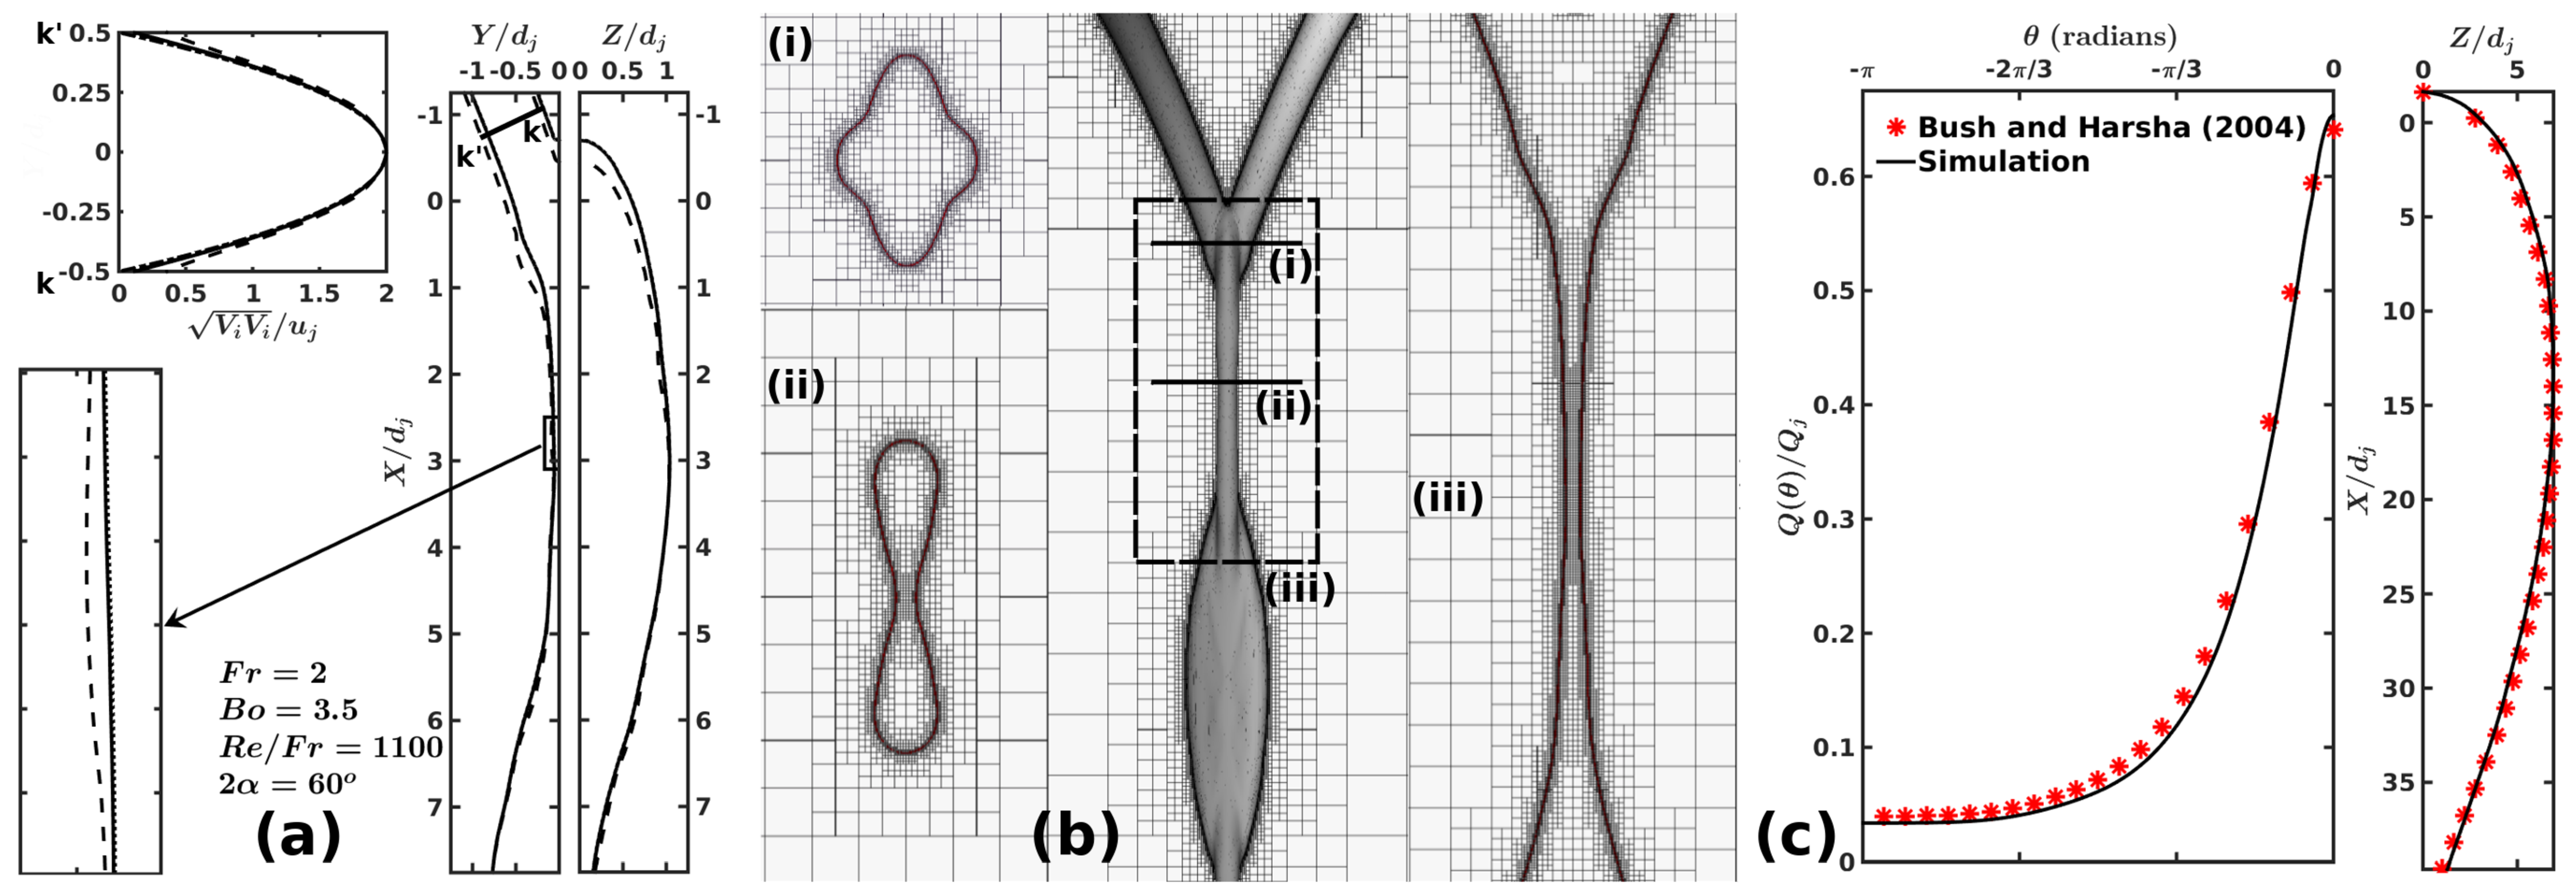
\includegraphics[width=\textwidth]{Figure2}
	\caption{(a) Mesh sensitivity analysis for a representative chain structure with the outer periphery and velocity profile near the inlet and (b) representation of the Adaptive Mesh Refinement (AMR) technique at critical locations.}
	\label{Figure::gisetal}
\end{figure*}
The collision of liquid jets has been studied in three-dimensional finite volume framework. Open source, time-dependent, multi-fluid, Navier-Stokes solver, Gerris is used for the current study \citep{Popinet2003}. The spatial discretization of the domain is undertaken using an octree-based structured hierarchical grid system, locally refined near the interface. Conventional mass and momentum conservation equations for incompressible flow have been solved in presence of the interface specific surface tension force ($\sigma \kappa$, where $\sigma$ is the surface tension coefficient and $\kappa$ denotes the curvature of the interface) and gravitational force density ($\rho g$, where $\rho$ is the density of fluid and $g$ acceleration due to gravity). The interface tracking is done using the Volume Of Fluid (VOF), a front capturing approach involving volume fraction of liquid, defined as $\Psi(x_i, t)$, at the spatial and temporal instance of $x_i$ and $t$ respectively. The density and viscosity for the study can be described using equation~\ref{Equation::general} in terms of a generic property $A$.
\begin{equation} \label{Equation::general}
A (\Psi) = \Psi A_1 + (1-\Psi)A_2 \: \: \:  \forall  \: A \in \{\rho, \mu\}
\end{equation}
The VOF approach is implemented in a two-step process of interface reconstruction (based on the values of $\Psi$ and piecewise linear interface construction scheme, PLIC) along with geometric flux computation and interface advection, shown in equation~\ref{Equation::vof}.
\begin{equation} \label{Equation::vof}
\frac{\partial \Psi}{\partial t} + \frac{\partial(\Psi V_i)}{\partial X_i} = 0
\end{equation}
Gerris uses second-order accurate time discretization of momentum and continuity equations with time splitting algorithm as proposed by \cite{Chorin1968}, whereby an unconditionally stable corrector predictor time marching approach is adopted. A multigrid solver is used for the solution of the resulting pressure-velocity coupled Laplace equation. The advection term of the momentum equation $\left(V_k\frac{\partial V_i}{\partial X_k}\right)$ is estimated using the Bell-Colella-Glaz second-order unsplit upwind scheme \citep{bell1989second}, which requires the restriction to be set up on the time step. Following \cite{popinet2009}, time step has been determined to satisfy Courant-Friedrich-Lewy (CFL) stability criteria of less than unity. The details of solution procedure can be found in the works of \cite{Popinet2003,popinet2009}.\\
\begin{figure}
	\centering
	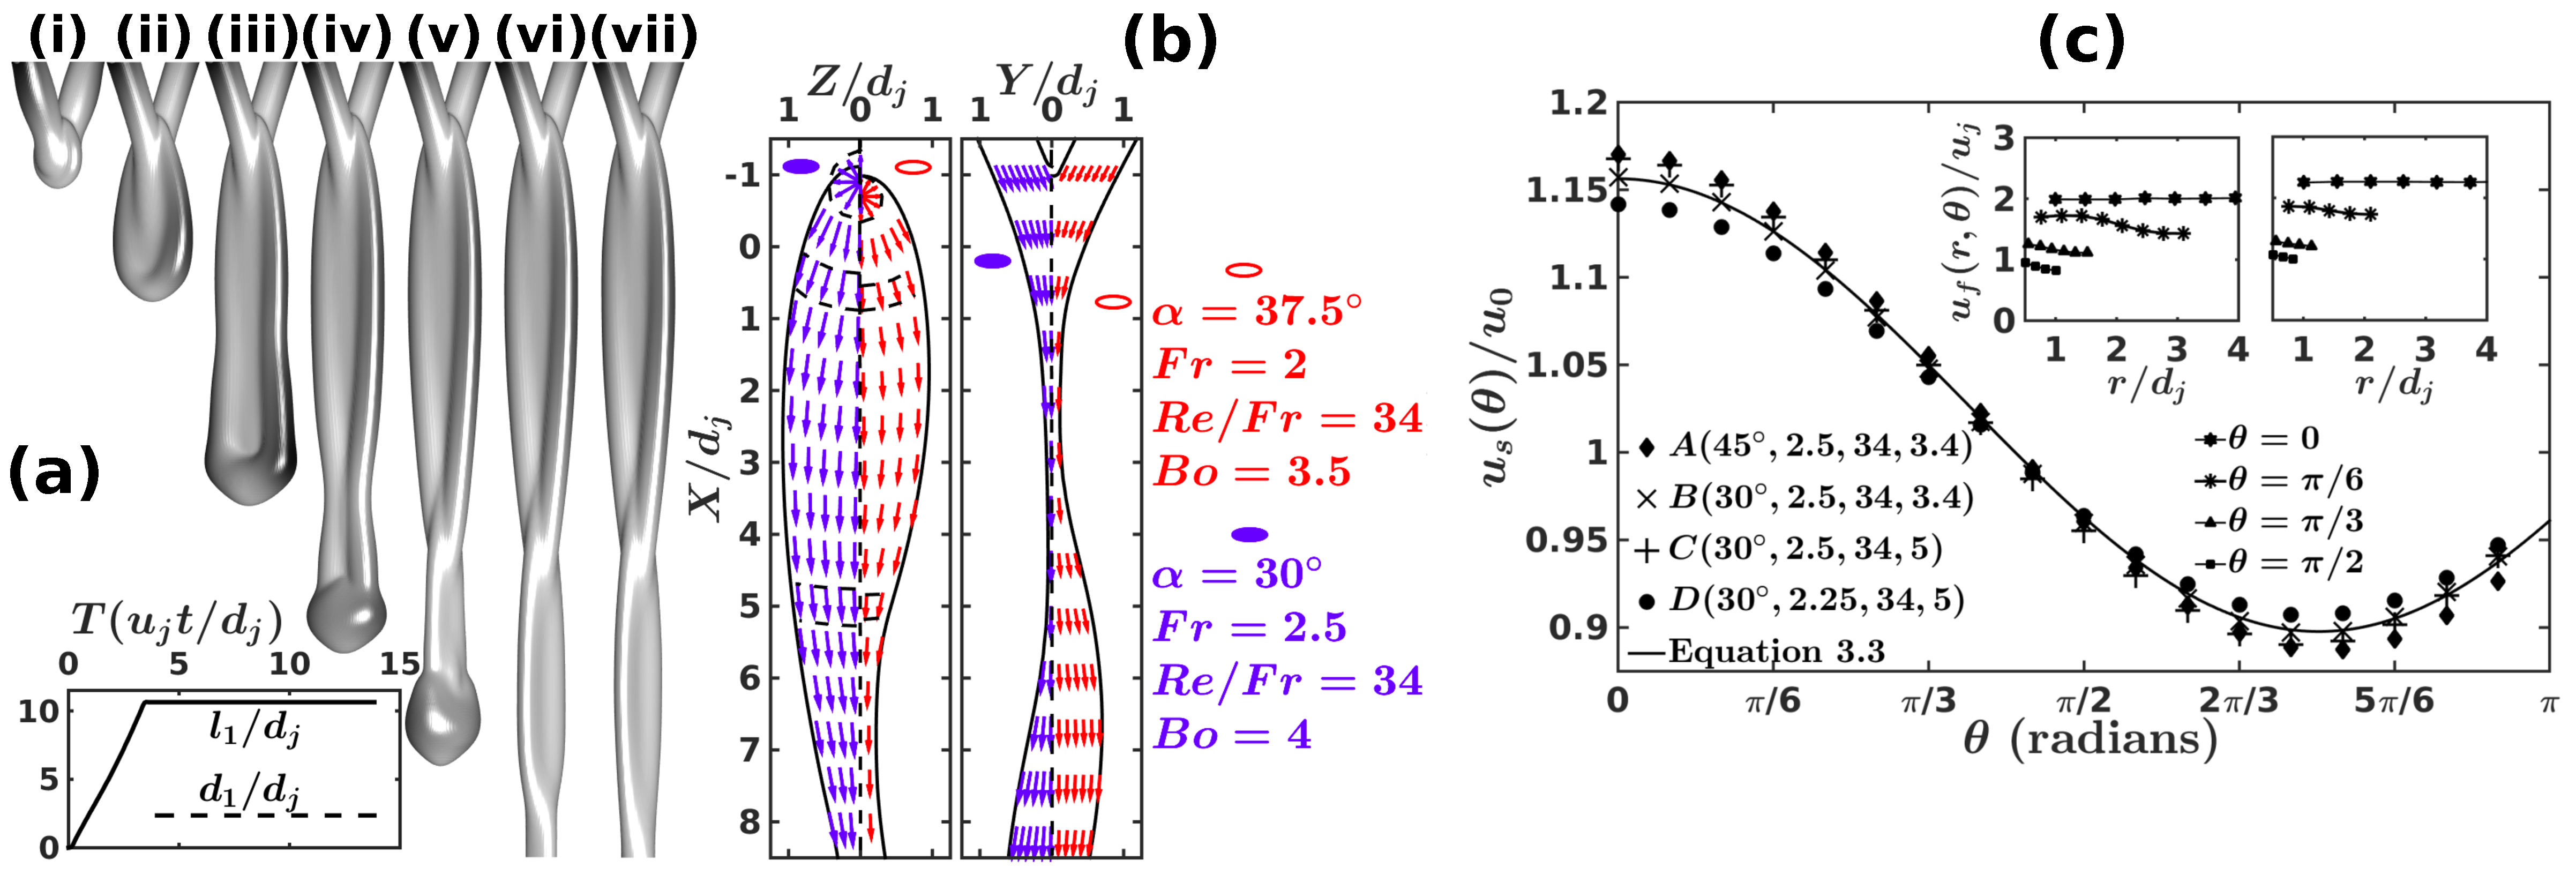
\includegraphics[width=\linewidth]{Figure3}
	\caption{Illustration of the validation of numerical model undertaken by comparison of (a) numerical interface and (b) liquid flux variation with the azimuthal angle, $\theta$. The numerically obtained results are superimposed with the respective experimental values obtained by \cite{bush2004collision}.}
	\label{Figure::validation}
\end{figure}
The computational domain is also illustrated in figure~\ref{Figure::schematic}(a) with parabolic inflow (suggested by \cite{choo2007effect} with average velocity, $u_j$) of jets (diameter, $d_j$ and impingement angle, $2\alpha$) and boundary outflow elsewhere. From the works of \cite{hasson1964thickness,choo2001parametric}, it can be shown that the thickness of liquid sheet follows $\frac{hr}{d_j^2} \sim 1$, for $2\alpha \in \{0,\pi/2\}$.  Here, $r$ is the radial direction originating from the collision point of the jets and $h$ is the measurement of the thickness of the film produced. We maintained $\frac{d_j}{\delta l} \sim 10\frac{r_{max}}{d_j}$ to choose minimum cell size $\left(\delta l\right)$ and perform Grid Independence Study (GIS). The factor of 10 is included to have at least 10 grid points \citep{ling2015multiscale} across the smallest length scale for the structure to avoid breakage of sheet \citep{chen2013high}. To obtain good liquid film resolution, $\delta l$ is varied to match the above-mentioned criteria. In one representative simulation, we show the effect of variation of $\delta l$, in figure~\ref{Figure::gisetal} (a), on sheet profile and velocity pattern of the jet. It can be observed that at $\frac{d_j}{\delta l}$ = 102.4, well resolved film is obtained with acceptable computational cost ($\sim 50\%$ less than $\frac{d_j}{\delta l}$ = 204.8). Mesh structure around different critical parts of the chain is shown in figure~\ref{Figure::gisetal}(b) which establishes sufficiency of grid points even inside smallest thickness of the film. To check the accuracy of the developed mesh structure, results from simulations are compared with experimental observations of sheet profile reported by \cite{bush2004collision} in figure~\ref{Figure::validation}(a). So as to get quantitative validation, the variation of liquid volume flux inside the sheet is also plotted in figure~\ref{Figure::validation}(b) along with \cite{bush2004collision}. In both the cases, matching between present numerical simulations and pioneering experimental result by \cite{bush2004collision} provides confidence for the numerical understanding of the phenomenon, in our work. Further, on performing non-dimensional analysis, it can be observed that Froude number $\left(Fr = \frac{u_j}{\sqrt{gd_j}}\right)$, Bond number $\left(Bo = \frac{\rho gd_j^2}{\sigma}\right)$ and ratio between Reynolds number and jet Froude number $\left(Re/Fr = \frac{\rho\sqrt{gd_j^3}}{\mu}\right)$ govern the shape and sizes of different links in the fluid chain structure. In our next section, a detailed study of the formation of the chain is presented based on above non-dimensional numbers.
\section{Collision and sheet formation}
\begin{figure*}
	\centering
	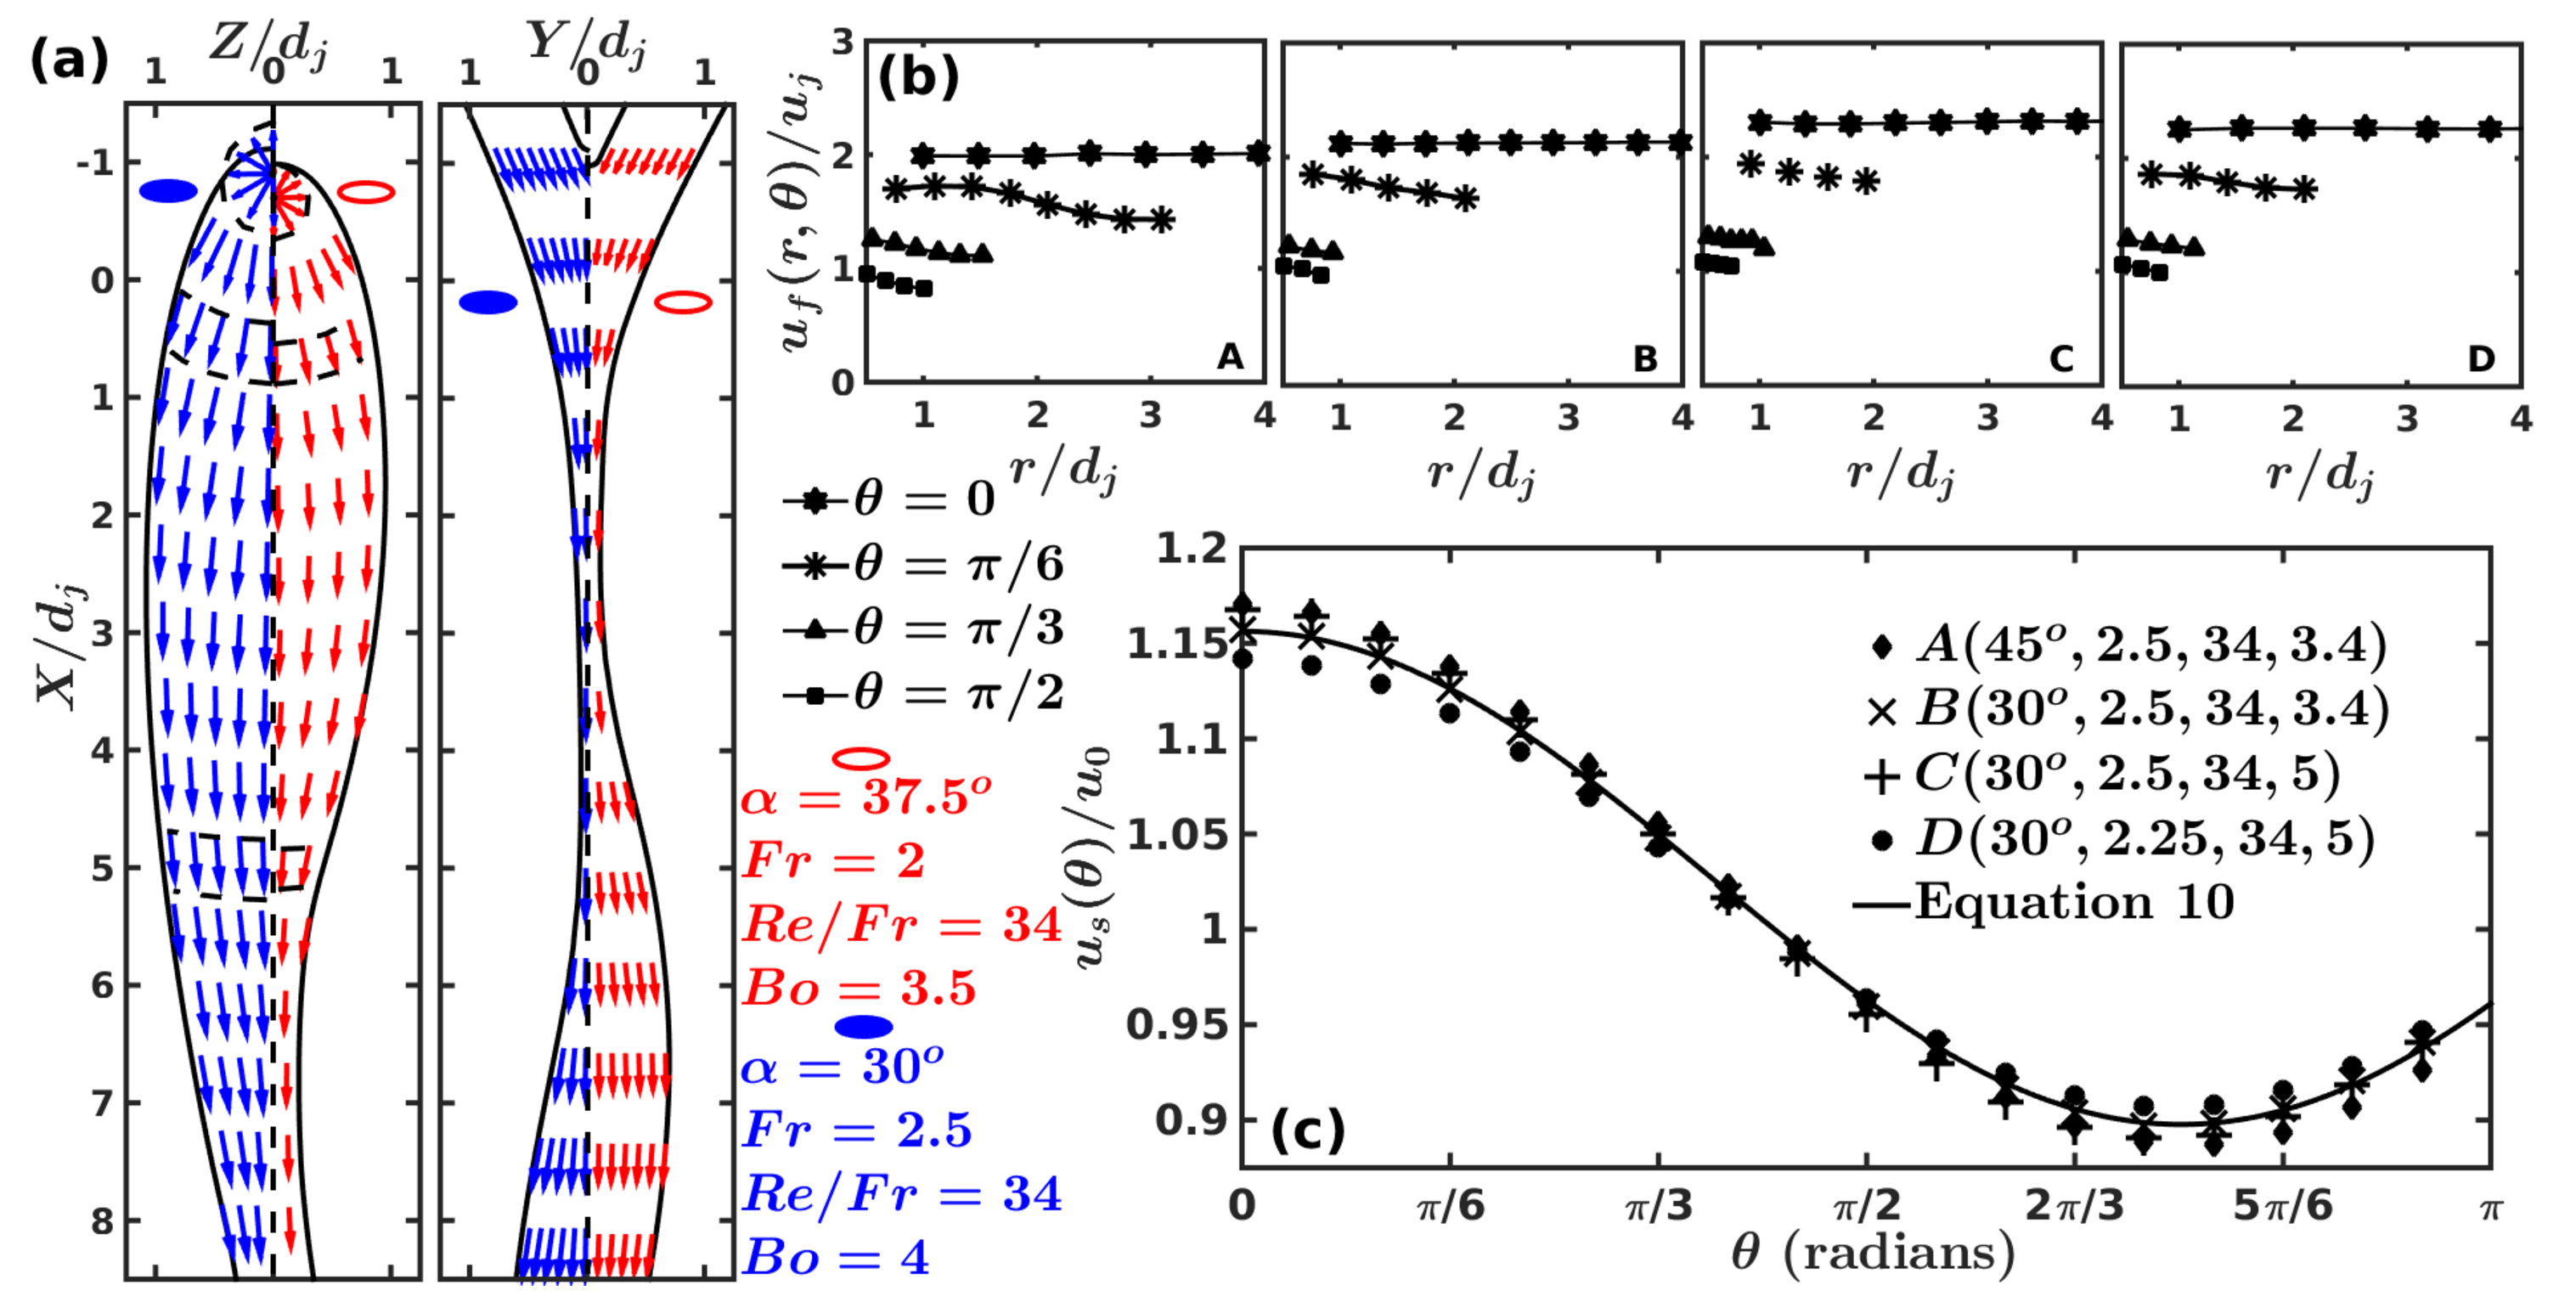
\includegraphics[width=\linewidth]{Figure4}
	\caption{Formation of the liquid chain due to the collision of laminar jets. The figure illustrates the transient period through the temporal advancement from (a) pre-collision symmetric jets to $T (\frac{u_jt}{d_j}) = $ (b) 1.5, (c) 4, (d) 5, (e) 5.5, (f) 6.5, (g) 8.5, (h) 14.5, (i) 18.5  and (j) 20. The variation of $d_1$ and $l_1$ with time is shown in inset ($\alpha$, $Fr$, $Re/Fr$, $Bo$ = 30\degree, 2.5, 34, 5). The video for this figure is added as a supplementary material.}
	\label{Figure::temporal}
\end{figure*}
As the laminar liquid jets collide, a thin sheet bounded by thicker rims is formed in the median plane, perpendicular to the axes of the jets. In this section, the formation of chain structure due to the collision of liquid jets is discussed. Figure~\ref{Figure::temporal} shows temporal evolution of the fluid sheet when the two jets (shown in figure~\ref{Figure::temporal}(a)) collide. The fluid parcels are dispatched radially outwards from the point of impingement. This along with net inertia of jets and gravity results in a bay leaf like sheet as shown in figures~\ref{Figure::temporal}(b) and~\ref{Figure::temporal}(c). Present zone of consideration lies in 0.5 $< Fr <$ 4, where gravity plays a major role unlike \cite{bush2004collision,bremond2006atomization}. In absence of surface tension or at very high Weber number, the sheet keeps on expanding (figures~\ref{Figure::temporal}(d) and~\ref{Figure::temporal}(e)), leading to the formation of the open rim structures \citep{taylor1960formation,chen2013high}. However, due to the action of the surface tension, the sheet stops expanding and the two rims at the periphery undergo a second oblique collision (figure~\ref{Figure::temporal}(f)) at an angle smaller than the initial collision (figure~\ref{Figure::temporal}(b)). After the secondary impingement, similar to figure~\ref{Figure::temporal}(c), a flow biased sheet begins to develop (figure~\ref{Figure::temporal}(g)). Formation of this second link has no effect on the characteristics features of the primary link as the sheet speed is supercritical \citep{bush2004collision}, and therefore can be independently studied. Temporal advancement results in the formation of a full-fledged secondary link as shown in figures~\ref{Figure::temporal}(h) to~\ref{Figure::temporal}(j). It must be noted that the plane of formation of this sheet is orthogonal to that of the primary link and therefore the secondary link shares the same plane as the axes of the jets. The process continues and a series of mutually orthogonal links are obtained, successively reducing in size until a long single liquid jet is formed \citep{bush2004collision}. After the initial transients, as seen from figure~\ref{Figure::temporal} and its inset, the links become steady (non-dimensionalized time, $T \left(\frac{u_jt}{d_j}\right) = $ 8.5 as representation in primary link), which has been analyzed further. \\
\begin{figure*}
	\centering
	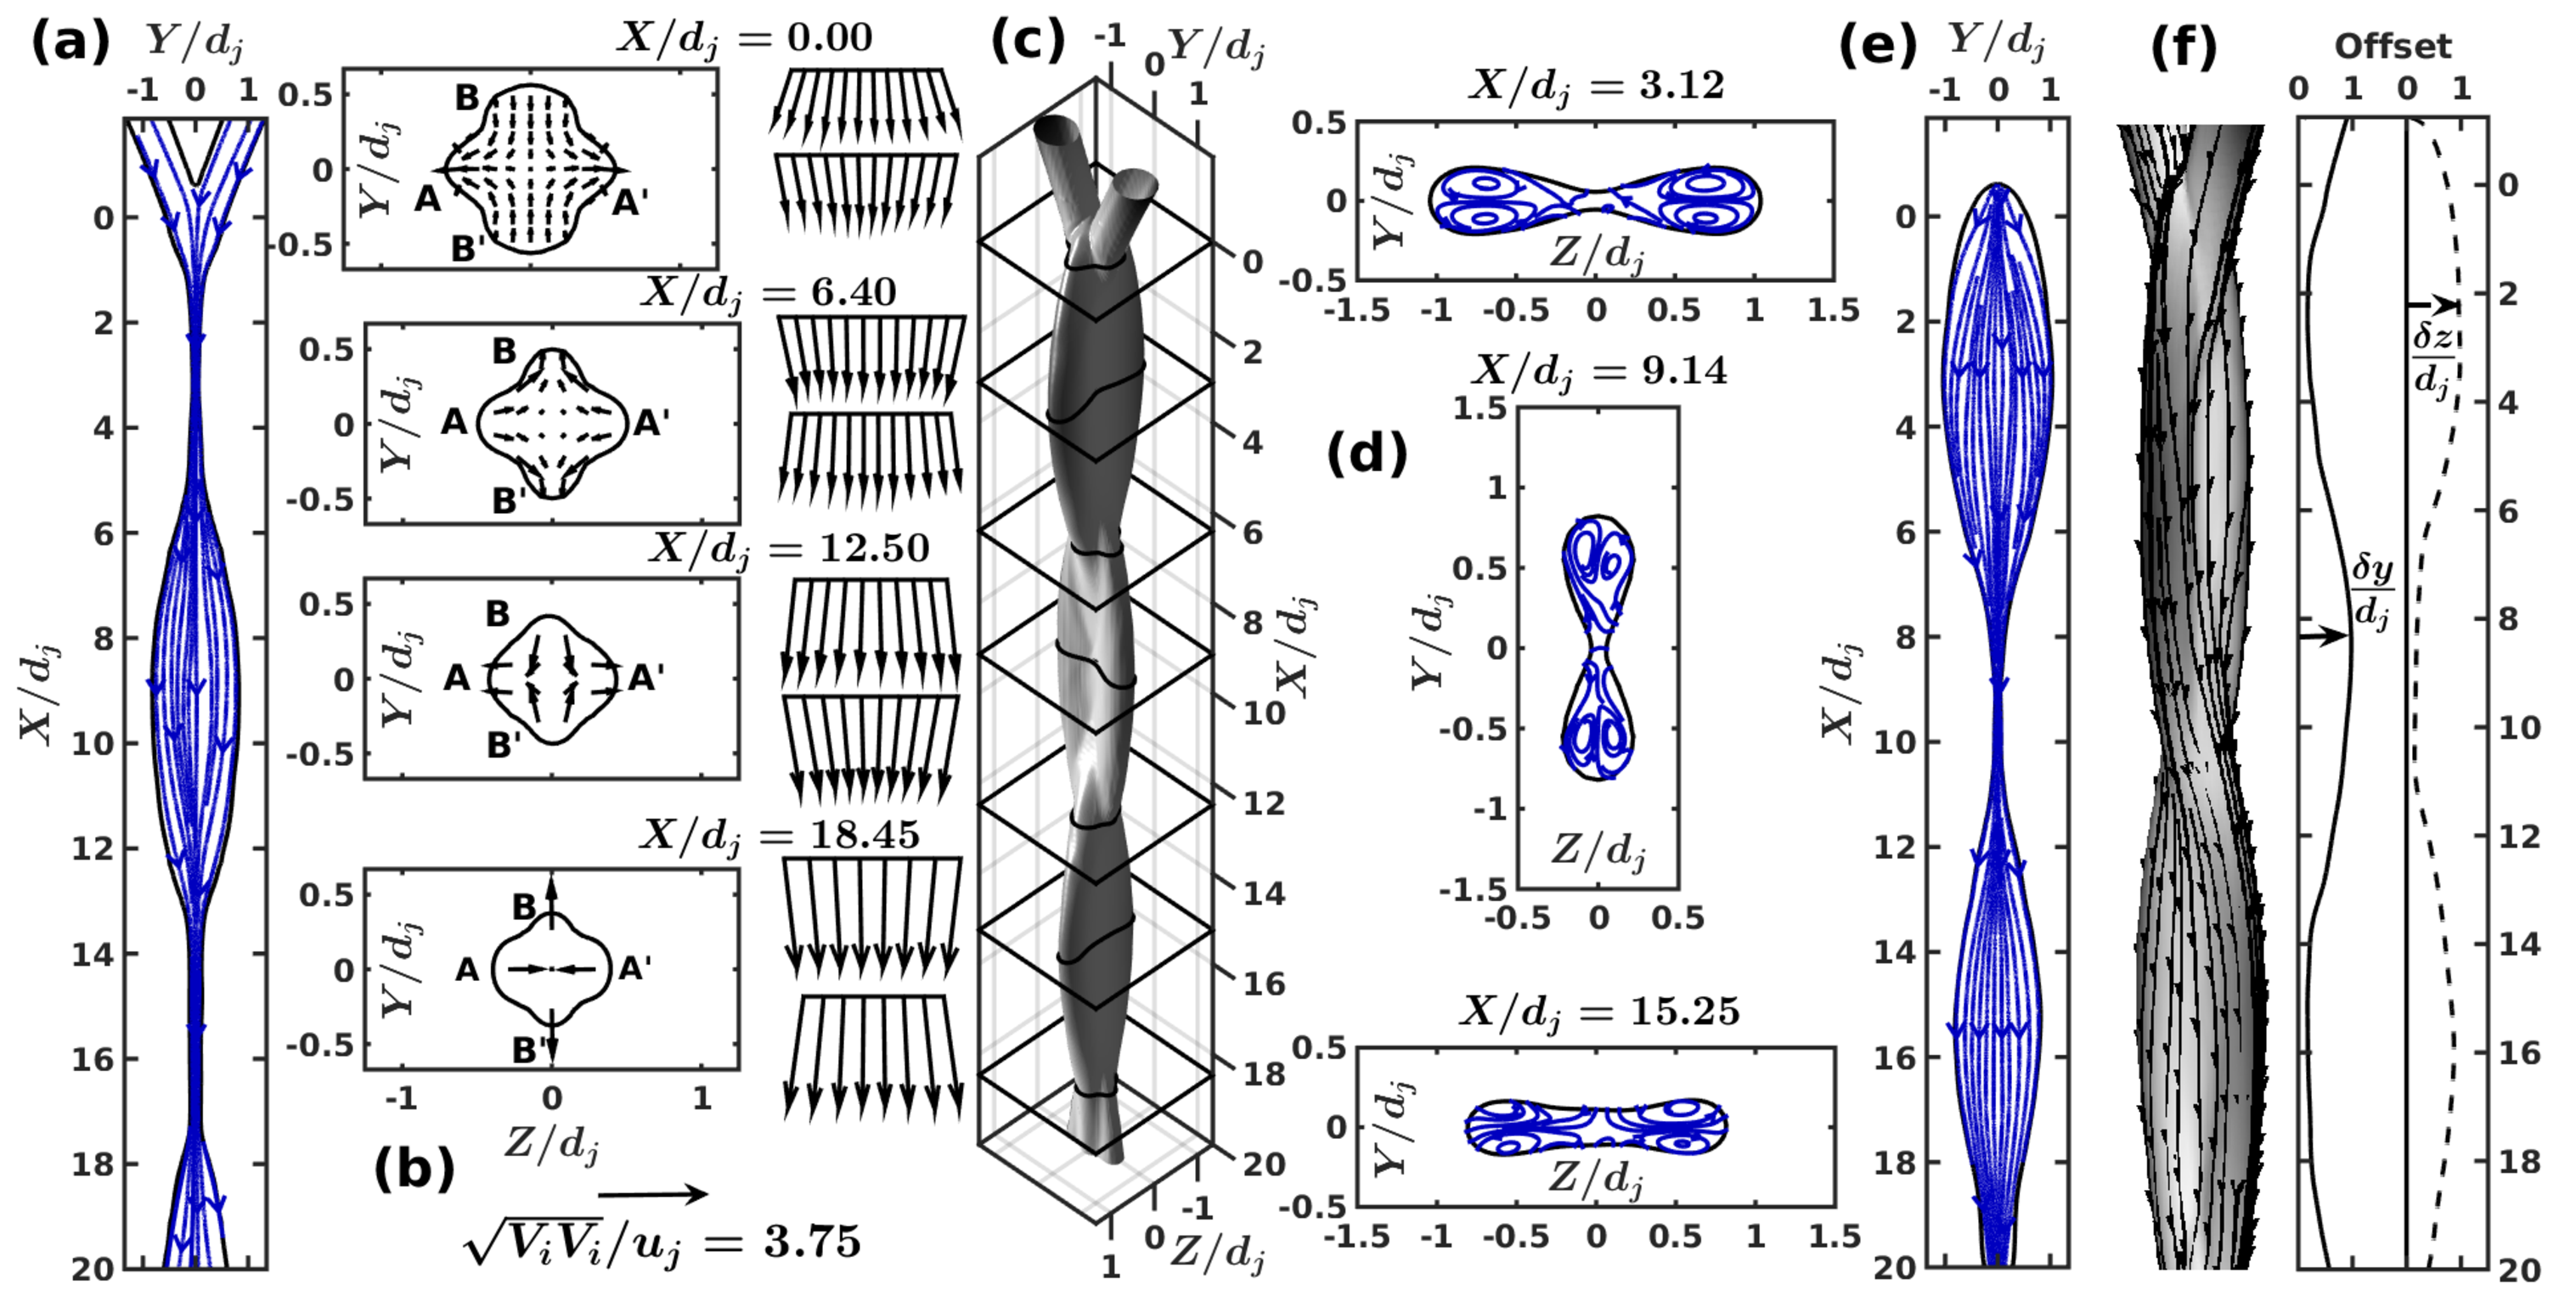
\includegraphics[width=\linewidth]{Figure5}
	\caption{Flow kinematics of the fluid parcels: (a) velocity vector field for two representative cases, (b) variation of velocity in the radial direction for four representative cases and (c) their radially averaged sheet velocity $\left(u_s(\theta)\right)$, non-dimensionalized with the average sheet velocity $\left(u_0\right)$ along the azimuthal direction in the sheet. The parameters identifying the identity of the cases follow ($\alpha$, $Fr$, $Re/Fr$, $Bo$).}
	\label{Figure::velocityVectors}%\vspace{-2mm}
\end{figure*}
Jets progress towards each other and collide at a point in the median sheet plane to form a sheet bounded by leaf-like rims. Fast moving, the thin sheet possess radial velocity pattern emerging from a stagnation point, $\delta_\pi$ higher than the impingement location. \cite{inamura2014effect} have established $\delta_\pi = \lambda d_j/(2\sin\alpha)$, where the factor $\lambda$ is a function of the impingement angle. It needs to be noted that $\delta_\pi$ changes its value, depending upon the angle of impingement and can be taken as a parameter. Considering $\delta_\pi$ and velocity vectors obtained from numerical simulations for two sets of non-dimensional numbers, flow pattern inside the sheet is reported in figure~\ref{Figure::velocityVectors}(a). It can be observed that velocity vectors follow a self-similar smooth path, as traced by sheet boundary. An increase of sheet span can be also noticed from the figure for a higher velocity of impacting jets. An effort has been made to observe the steady average flow $\left(u_f(r,\theta)\right)$ across the thickness of the sheet at a given radial and azimuthal point. It can be expressed as equation~\ref{Equation::uf}, where $Y$ is the coordinate direction parallel to link's thickness. 
\begin{equation}\label{Equation::uf}
u_f(r,\theta) = \int_{0}^{1}\sqrt{V_iV_i}d(Y/h)
\end{equation}
$V_i$ denotes the velocity field in Cartesian-tensor notation and $\sqrt{V_iV_i}$ is the total magnitude of the velocity given by $\sqrt{V_r^2 + V_\theta^2 + V_z^2}$. Azimuthal and radial velocities are considered here to accommodate spread of fluid streams, forming chain and subsequent links in orthogonal planes. The variation of $u_f(r,\theta)$ along radial plane at different azimuthal angles have been shown in figure~\ref{Figure::velocityVectors}(b). It can be observed that the order of change in the fluid velocity across the radial distance from the point of impact is less than the change across the azimuthal direction (also discussed by \cite{choo2002velocity}). Further, sheet velocity $\left(u_s(\theta)\right)$ along a radial plane has been also obtained by integrating $u_f(r,\theta)$ as:
\begin{equation}\label{Equation::us}
u_s(\theta) = \int_{0}^{1}u_f(r,\theta)d(r/r_{max})
\end{equation} 
Upon non-dimensionalization of sheet velocity with its average $\left(u_0\right)$, a self-similar behavior in azimuthal direction is observed for a wide diversity of non-dimensional parameters reported in figure~\ref{Figure::velocityVectors}(c). In this figure, four arbitrarily chosen parameters are shown which adhere to a functional relationship of $u_s(\theta)$ in the following fashion: 
\begin{equation}\label{Equation::usu0}
\frac{u_s(\theta)}{u_0} = 1.03 + 0.13\cos\left(\frac{4.18\theta}{\pi}\right)
\end{equation}
It needs to be noted that equation~\ref{Equation::usu0} is valid for a large range of non-dimensional numbers explored in the present study, forming stable chain structure (0\degree $< \alpha \le$  45\degree, $Fr \sim$ 1, $Bo \sim$ 1 and 10 $\le Re \le$ 2300). Once the average sheet velocity exceeds a critical value, the chain structure is no longer stable as the  Kelvin - Helmholtz instability kicks in \citep{villermaux2002life}. \\
\begin{figure*}
	\centering
	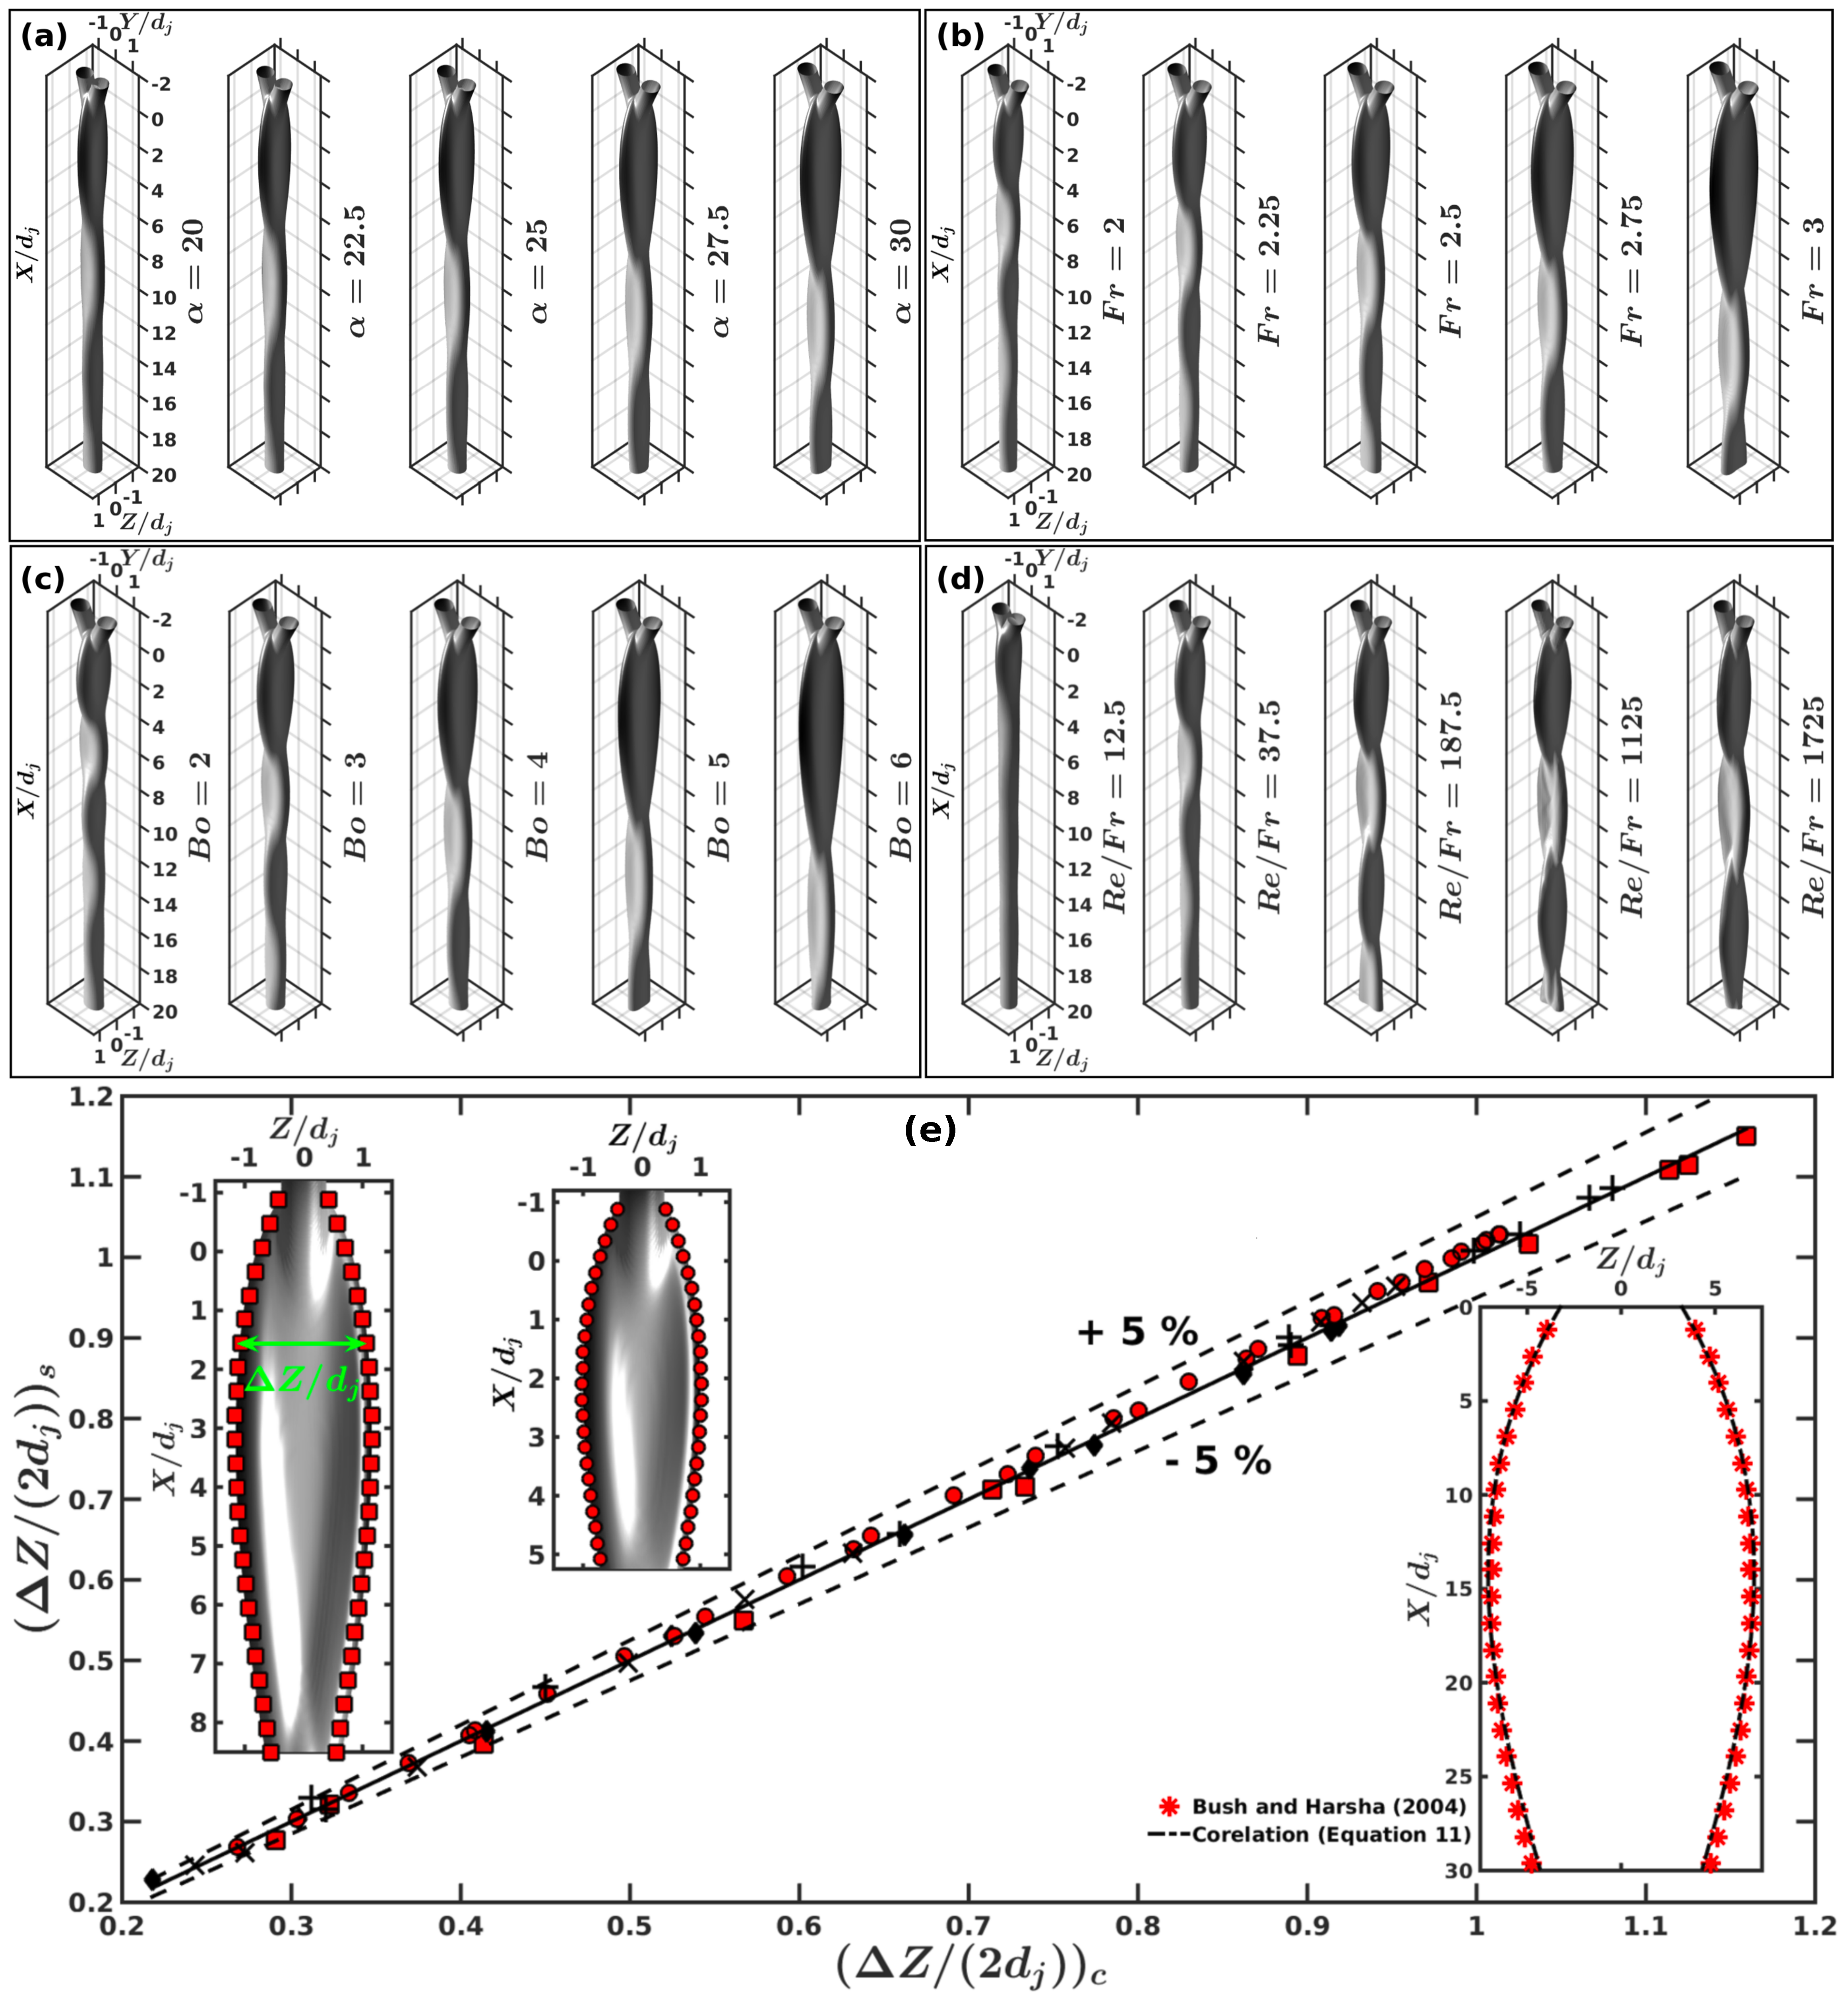
\includegraphics[width=\linewidth]{Figure6}
	\caption{Three dimensional velocity field for ($\alpha, Fr, Re/Fr, Bo$) = (30$\degree$, 2, 1125, 3.4) with (a) XY plane streamlines, (b) velocity vector field in the YZ plane at different collision locations, (c) the three dimensional stable chain structure, (d) streamlines at maximum link widths in the YZ plane and (e) XZ plane streamlines.}
	\label{Figure::streamDetails}
\end{figure*}
\begin{figure}
	\centering
	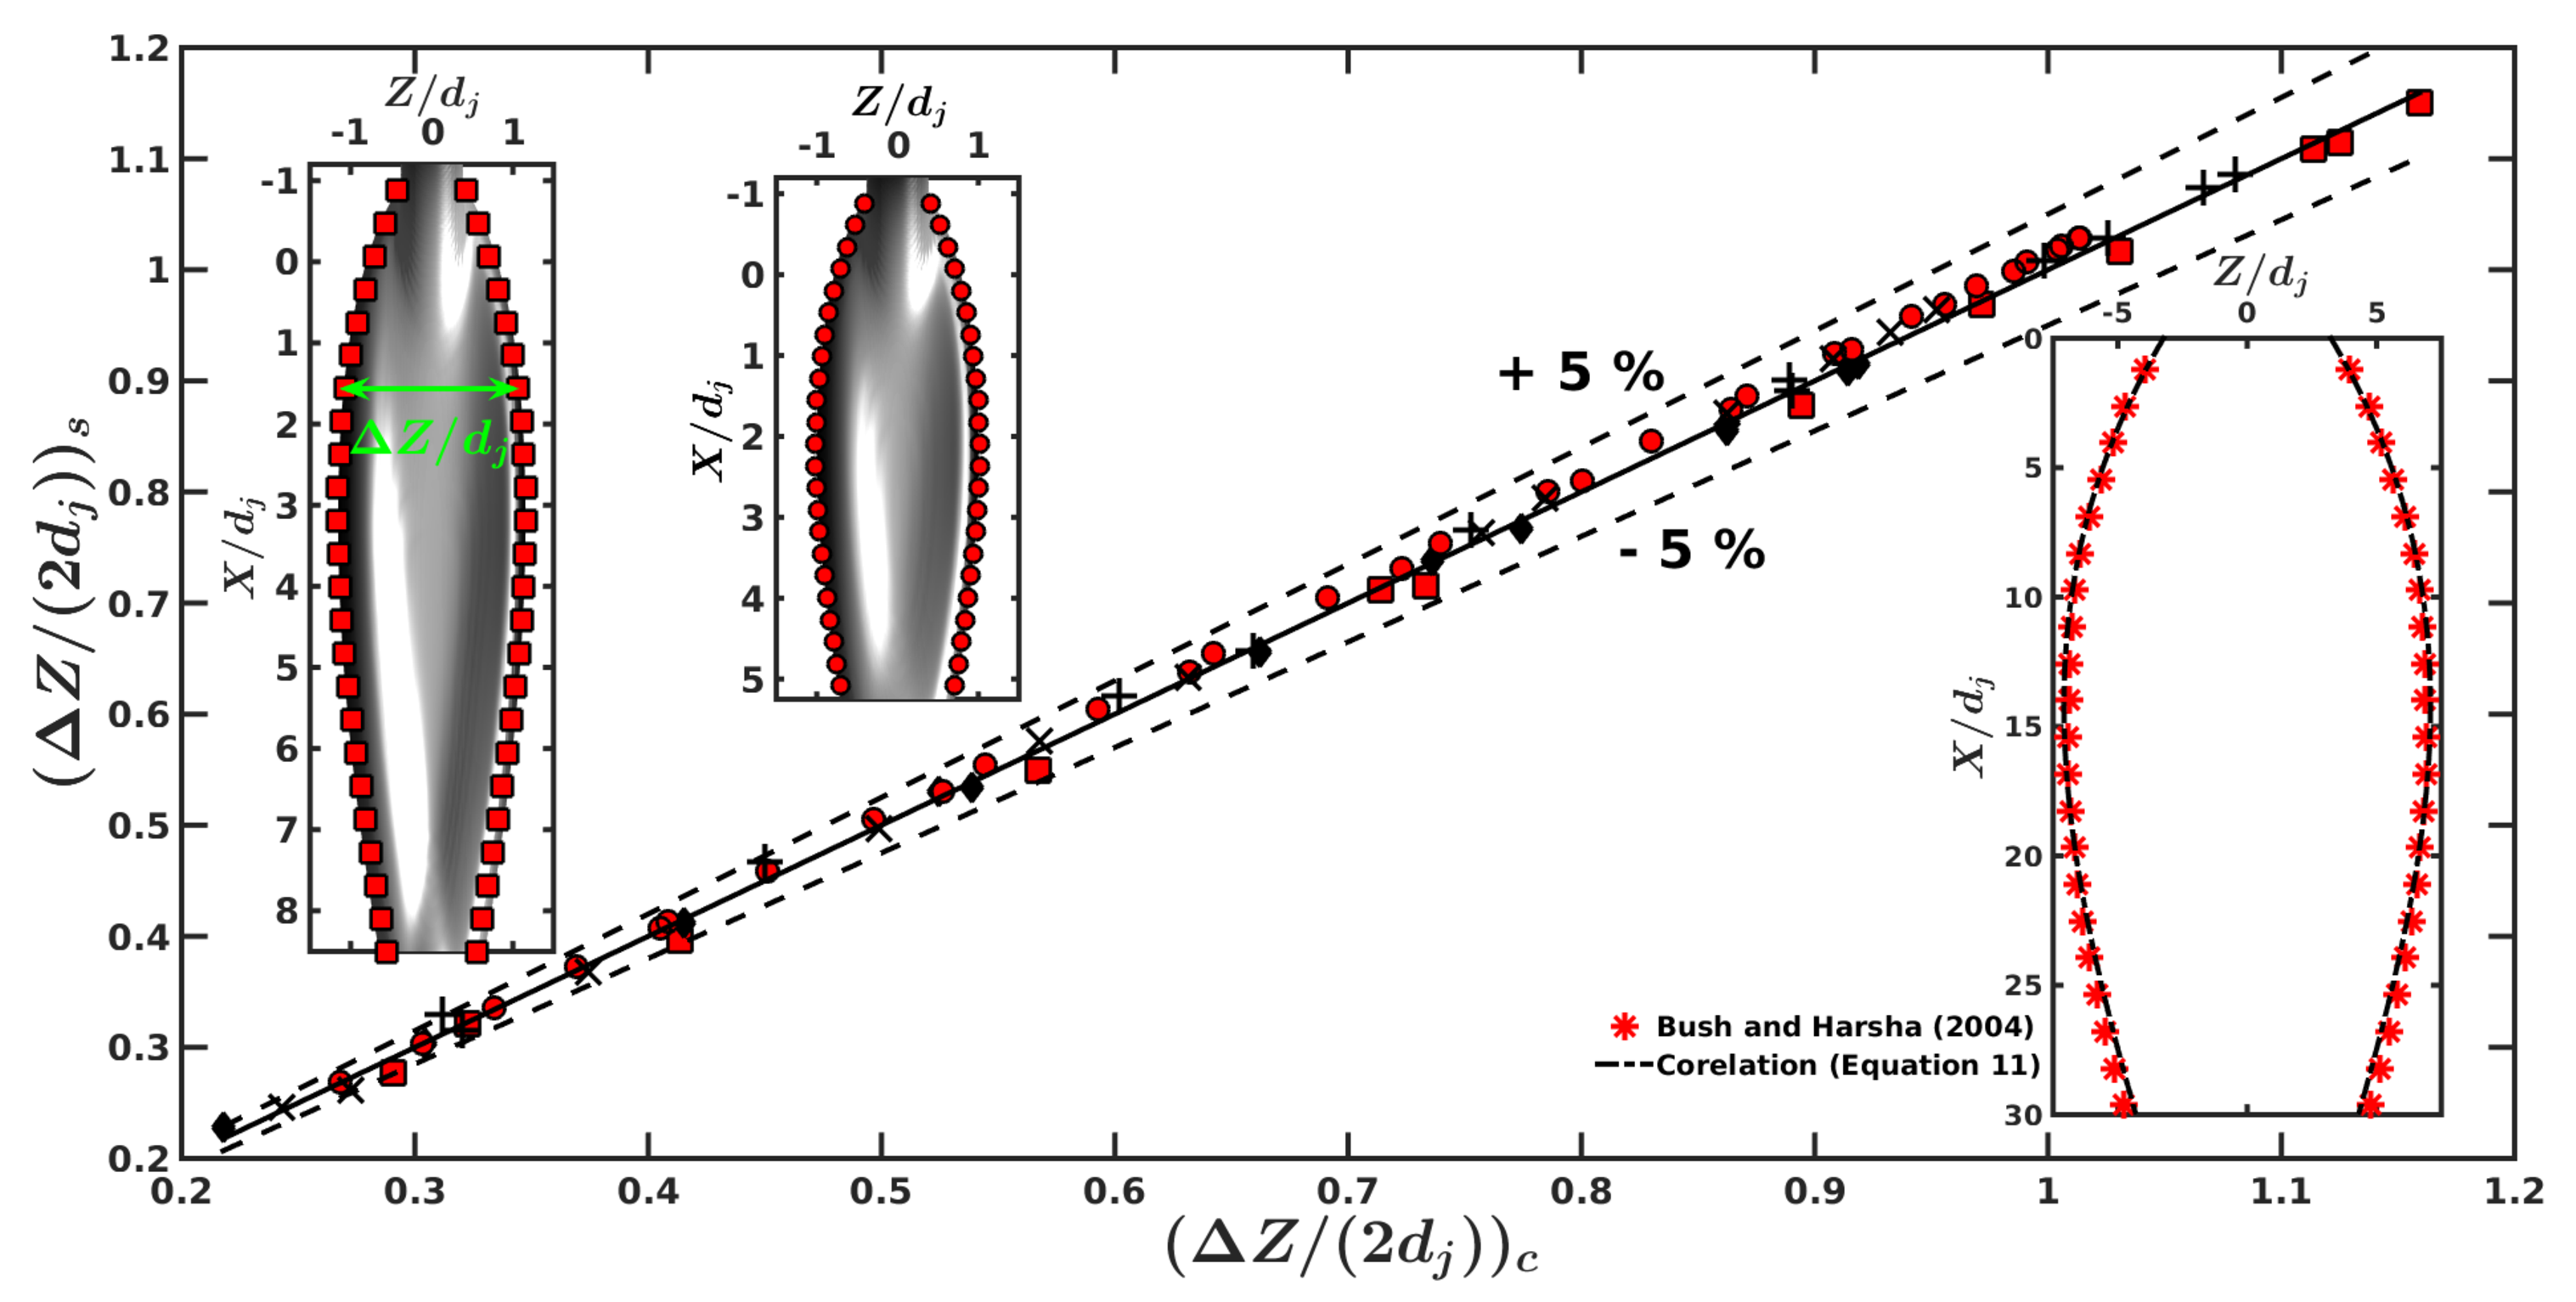
\includegraphics[width=\linewidth]{Figure7}
	\caption{Three dimensional streamlines embedded on the chain structure illustrating the twist incurred as they traverse through the region of subsequent collisions for $\alpha$ = $30\degree$, $Fr$ = 2, $Bo$ = 3.4 and (a) $Re/Fr$ = 1750 and (b) $Re/Fr$ = 34. The figures in inset show the offset ($\delta y$ from XZ plane and $\delta z$ from XY plane) of the streamline at the extreme end of the chain structure as it moves downstream with the flow for the corresponding cases.}
	\label{Figure::stream3D}
\end{figure}
An overall consideration of the three-dimensional chain structure (figure~\ref{Figure::streamDetails}(c)) allows us to obtain velocity patterns at different axial locations. The streamlines follow steadily the phase contour boundary, with those inside the chain structure going in trajectories similar to the outer boundary as shown in figures~\ref{Figure::streamDetails}(a) and~\ref{Figure::streamDetails}(e). Figure~\ref{Figure::streamDetails}(b) puts an effort towards highlighting velocity vectors at primary, secondary and tertiary links. One can observe from figure~\ref{Figure::streamDetails}(b) that the spread of liquid influence at collision planes is reducing continuously as $X/d_j$ increases.  At the primary ($X/d_j$ = 0) and tertiary ($X/d_j$ = 12.5) collision points, the liquid jets and rims respectively converge onto themselves ($Z/d_j$ = 0) marked by retracting velocity field, whereas the liquid sheet grows ($Y/d_j$ = 0) in the Z direction, marked by an expanding velocity field. Trends opposite to these are obtained at the secondary ($X/d_j$ = 6.40) and quaternary ($X/d_j$ = 18.45) collision planes where a retracting velocity field is present at $Y/d_j$ = 0 and expansion happens at $Z/d_j$ = 0. This leads to the formation of three visible orthogonal links in this case (figure~\ref{Figure::streamDetails}(c)). The velocity vector magnitudes go on increasing at each subsequent collision planes as the gravitational head is converted to dynamic head leading to narrowing of the extent of liquid phase boundary in the XZ plane. In the primary link, this converging-diverging trend of velocity vectors is continued from above the first collision point ($X/d_j$ = 0) to the plane where the extent of the link perpendicular to the net flow direction in the plane of the link is maximum ($X/d_j$ = 3.12). As illustrated in figure~\ref{Figure::streamDetails}(d), the streamlines at the location of maximum width imply that the component of velocity perpendicular to the liquid sheet phase boundary is zero ($\frac{d\Psi}{dn}$ = 0). This results in the formation of distinguished circulation patterns inside the lobes at the locations of the maximum extent ($X/d_j$ = 3.12, 9.14 and 15.25) corresponding to the three links visible in this case. Reduction of collision strength at different planes explains diminishing spans of the links, which can be also seen from sheet cross-sectional images (figure~\ref{Figure::streamDetails}(d)).\\
A characteristic twist can be found in streamlines (figure~\ref{Figure::stream3D}) as the flow propagates downstream through the locations of subsequent collisions. The twist occurs as the fluid parcels are restricted by surface tension to follow the chain's outer periphery. This twist is characterized by the offset of these streamlines from the two mutually orthogonal planes: the XY plane containing the axes of the liquid jets ($\delta z$) and the XZ median plane orthogonal to this one ($\delta y$). The offset of the most extreme streamline are shown in the inset of figure~\ref{Figure::stream3D} for two representative cases having different ratios of Reynolds Number and Froude Number ($Re/Fr$ = 1750 in figure~\ref{Figure::stream3D}(a) and $Re/Fr$ = 34 in~\ref{Figure::stream3D}(b)). The offset of all the streamlines from the XZ plane ($\delta y$) decreases continuously as the liquid jets approach each other (retracting velocity field as shown in figure~\ref{Figure::streamDetails}(b)). After the collision, two extreme streamlines in XZ and XY planes are depicted in the inset of figures~\ref{Figure::stream3D} (a) and~\ref{Figure::stream3D} (b). It is observed that $\delta y$ decreases continuously through the first link, but downstream of the second collision, the offset starts to increase, reaching the maxima at the location of the maximum width of the secondary link. The opposite trend is observed for the XY plane whereby the offset ($\delta z$) increases after the first collision continuously till the maximum width of the primary link and then decreases for the secondary link. These variations in the offset in streamlines show the presence of twist, which is prominent until viscous effects start dominating and only a single jet of liquid is left at the end of the chain structure (as shown in figure~\ref{Figure::stream3D}(b) beyond $X/d_j$ = 16). These viscous forces lead to dissipation of energy as the liquids jets (or rims for the post-primary link) collide with each other. It is clear from our discussions above that values of dimensionless numbers $\alpha$, $Fr$, $Bo$ and $Re/Fr$ determine the three-dimensional stable chain structures. The next section is devoted to analyzing such effects.
\section{Assessment of factors influencing chain structure}
\begin{figure*}
	\centering
	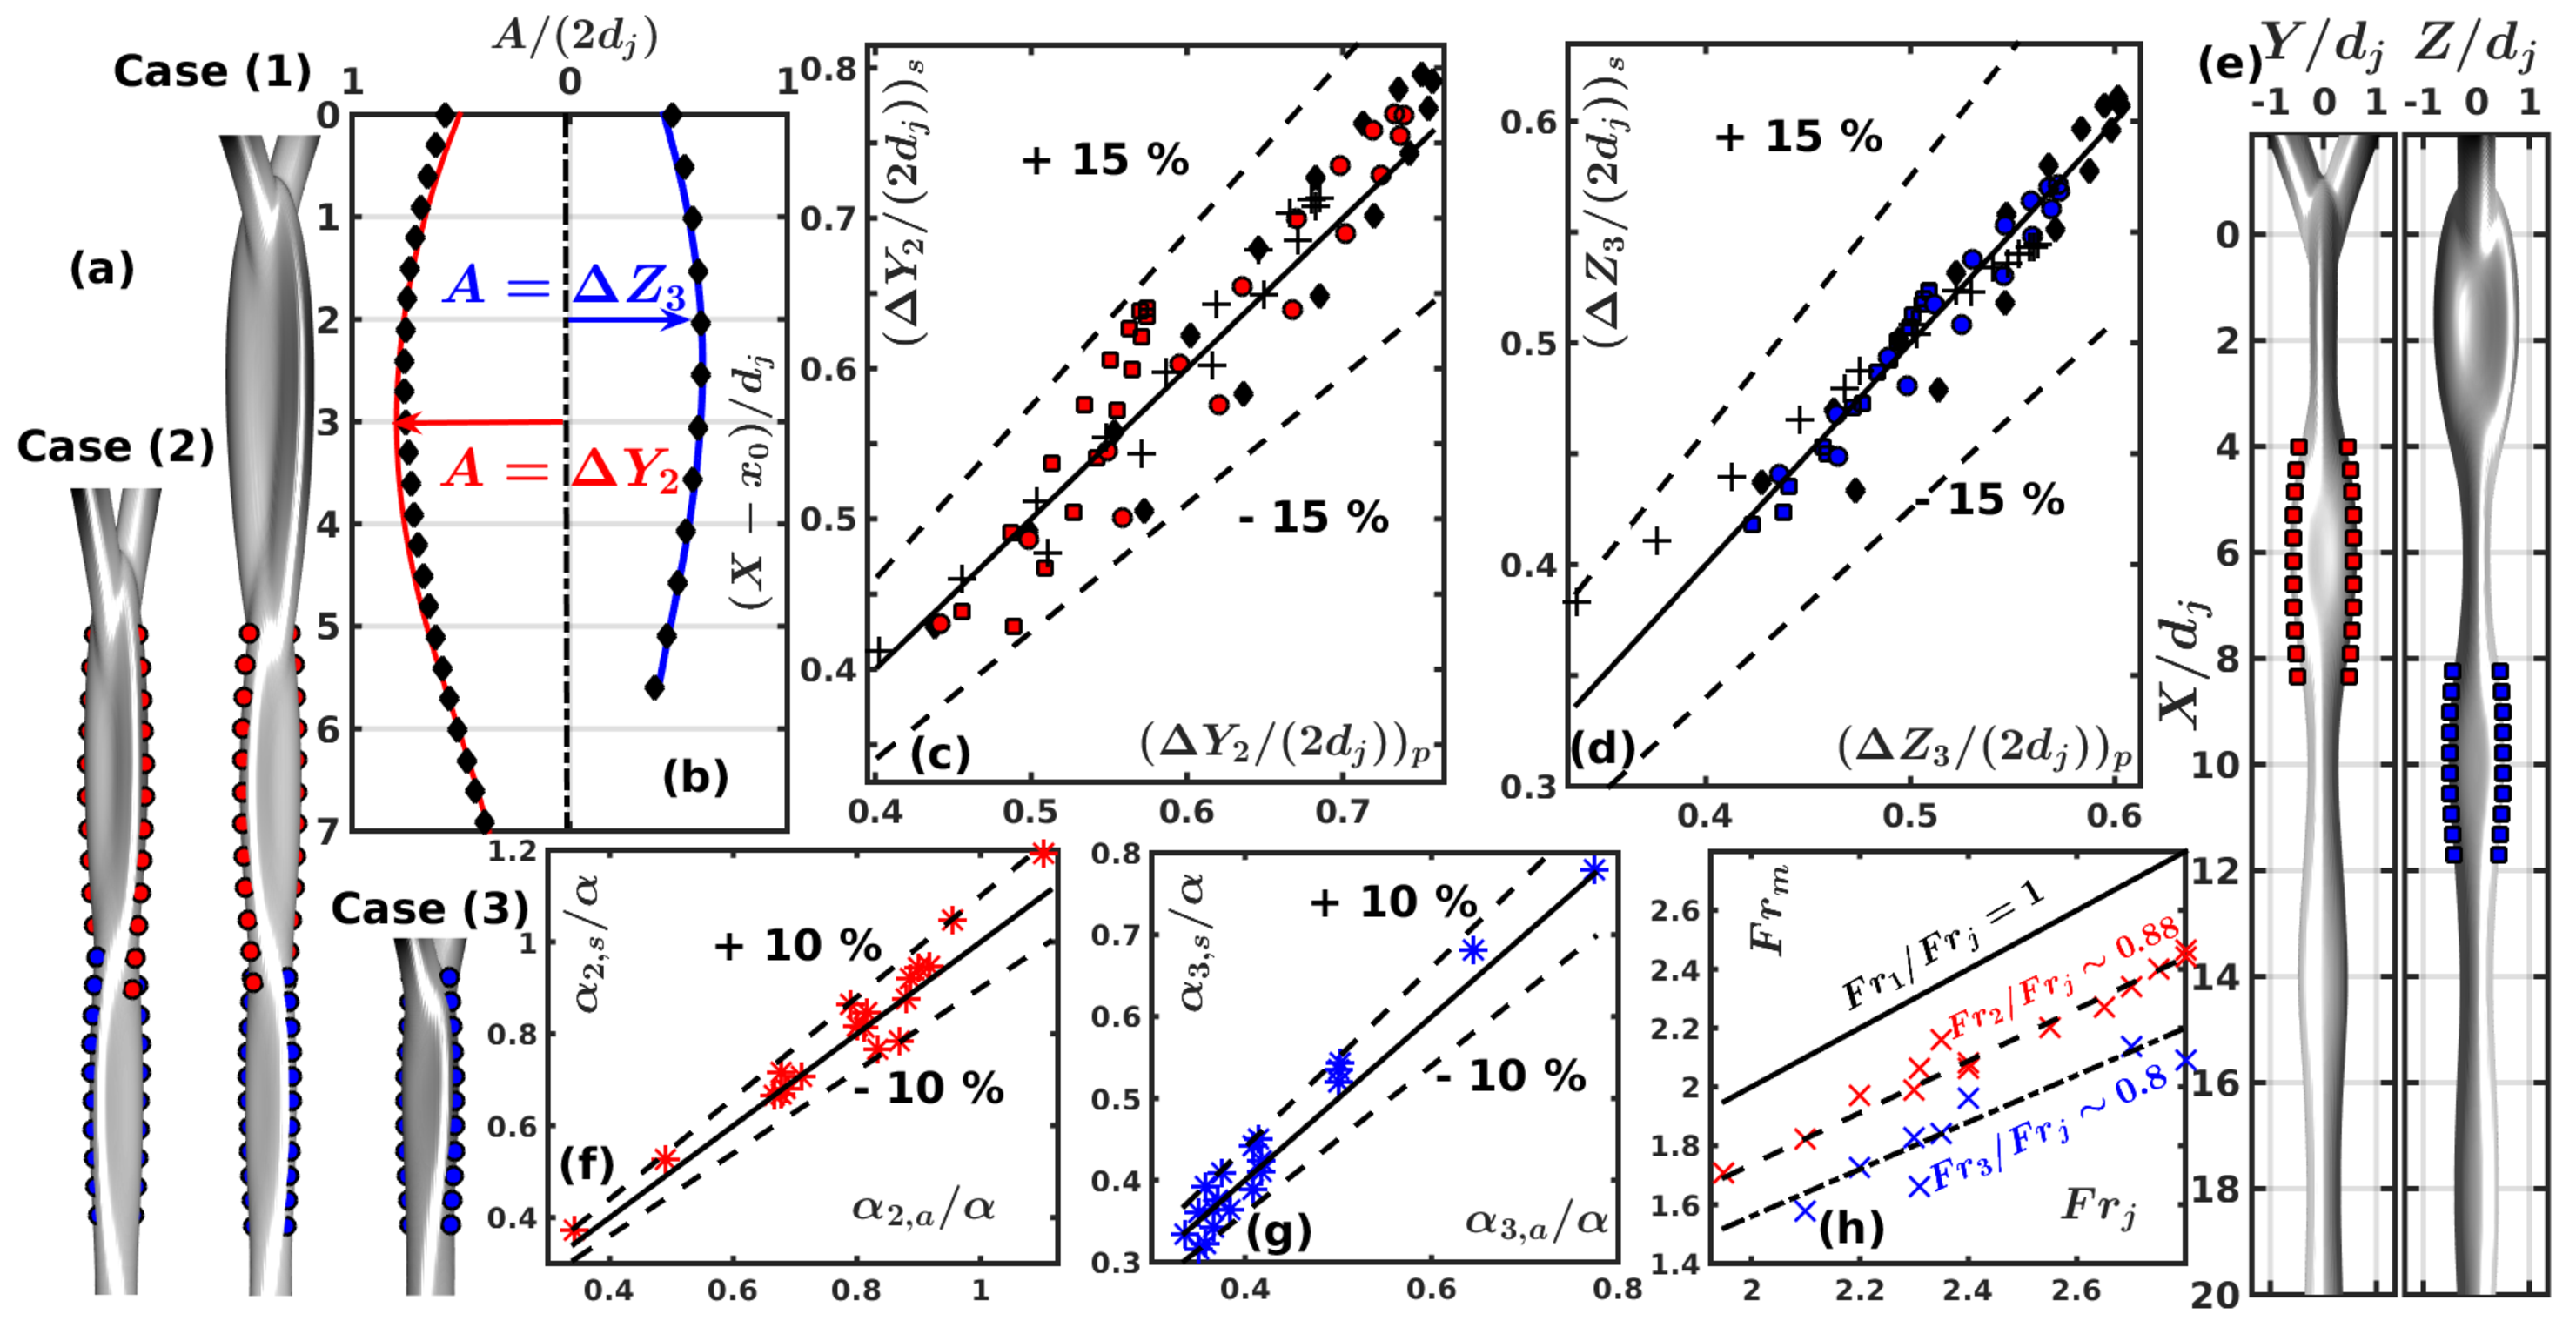
\includegraphics[width=\linewidth]{Figure8}
	\caption{High fidelity numerical simulations of liquid jets collision to form chain structure for variation of (a) $\alpha$ at $Fr$ = 2.5, $Bo$ = 4.57 and $Re/Fr$ = 34 (b) $Fr$ at $\alpha$ = 30$\degree$, $Bo$ = 3.4 and $Re/Fr$ = 34 (c) $Bo$ at $\alpha$ = 30$\degree$, $Fr$ = 2.5 and $Re/Fr$ = 34 and (d) $Re/Fr$ at $\alpha$ = 30$\degree$, $Fr$ = 2 and $Bo$ = 3.4.}
	\label{Figure::phaseContours}
\end{figure*}
Formation of the liquid sheet bounded by the rims is governed by inertia, viscous, buoyancy and surface forces apart from the angle of impingement between the jets ($\alpha$). The relative importance of these forces is described by the parameters $Fr$, $Bo$ and $Re/Fr$, as mentioned above. In this section, critical assessment of chain shapes is made for various non-dimensional numbers and impingement angles. \cite{yang2014liquid} acknowledged the importance of these parameters on collision process and formation of the first link. Figures~\ref{Figure::phaseContours}(a) -~\ref{Figure::phaseContours}(d) show numerical chain structure for a several sets of parameters $\alpha$, $Fr$, $Bo$ and $Re/Fr$. An increase in impingement angle leads to decrease of jet momentum in direction of gravity ($u_j\cos\alpha$) and a substantial increase in width of the sheet, keeping the length more or less intact (figures~\ref{Figure::phaseContours}(a)). Alternatively, as the jet momentum is increased (increase in $Fr$), the resulting links are bigger (figure~\ref{Figure::phaseContours}(b)) due to the fluid inertia. One can clearly see this effect is transmitted to the subsequent links as well. Further, the surface tension is a crucial entity which influences the expansion of the link. As the surface tension is decreased ($Bo$ increased), the link can expand until inertial and centrifugal forces balance it. This justifies obtaining larger links for higher values of $Bo$ as seen in figures~\ref{Figure::phaseContours}(c). As the surface tension is increased (low $Bo$ regime), the system tries to go towards the minimum surface energy decreasing the dimensions of the corresponding links (link in figure~\ref{Figure::phaseContours}(c) from $Bo$ = 6 to 2). Further, the collision of cylindrical jets and rims is also observed to be influenced by viscous dissipations. Decreasing the viscosity (increasing $Re/Fr$) leads to considerable increase in sheet dimensions but its effect saturates at lower ranges of liquid viscosities (figure~\ref{Figure::phaseContours}(d)). Effect of change in liquid viscosity dies down as inertia and surface tension overshadow its resistance to form similar shape and sizes of links. It can also be noticed that it is the viscous dissipations that result in the decrement in the size of subsequent links leading to a point where the sheet coalesces into a single jet of fluid. The effect is prominent in figure~\ref{Figure::phaseContours}(d) for $Re/Fr$ = 12.5.\\
Considering $\Delta Z$ is the rim to rim distance at a particular vertical location ($X$) of the symmetric sheet, a third order polynomial is used to fit ($R^2 >$ 0.975; $SSE <$ 0.01) the sheet shape for various influencing parameters. The functional form of the polynomial is as follows: 
\begin{equation}\label{Equation::correlation}
\frac{\Delta Z}{2d_j} = \sum_{n = 0}^{n = 3}p_n\left(\frac{X}{d_j}\right)^n
\end{equation}
\begin{figure*}
	\centering
	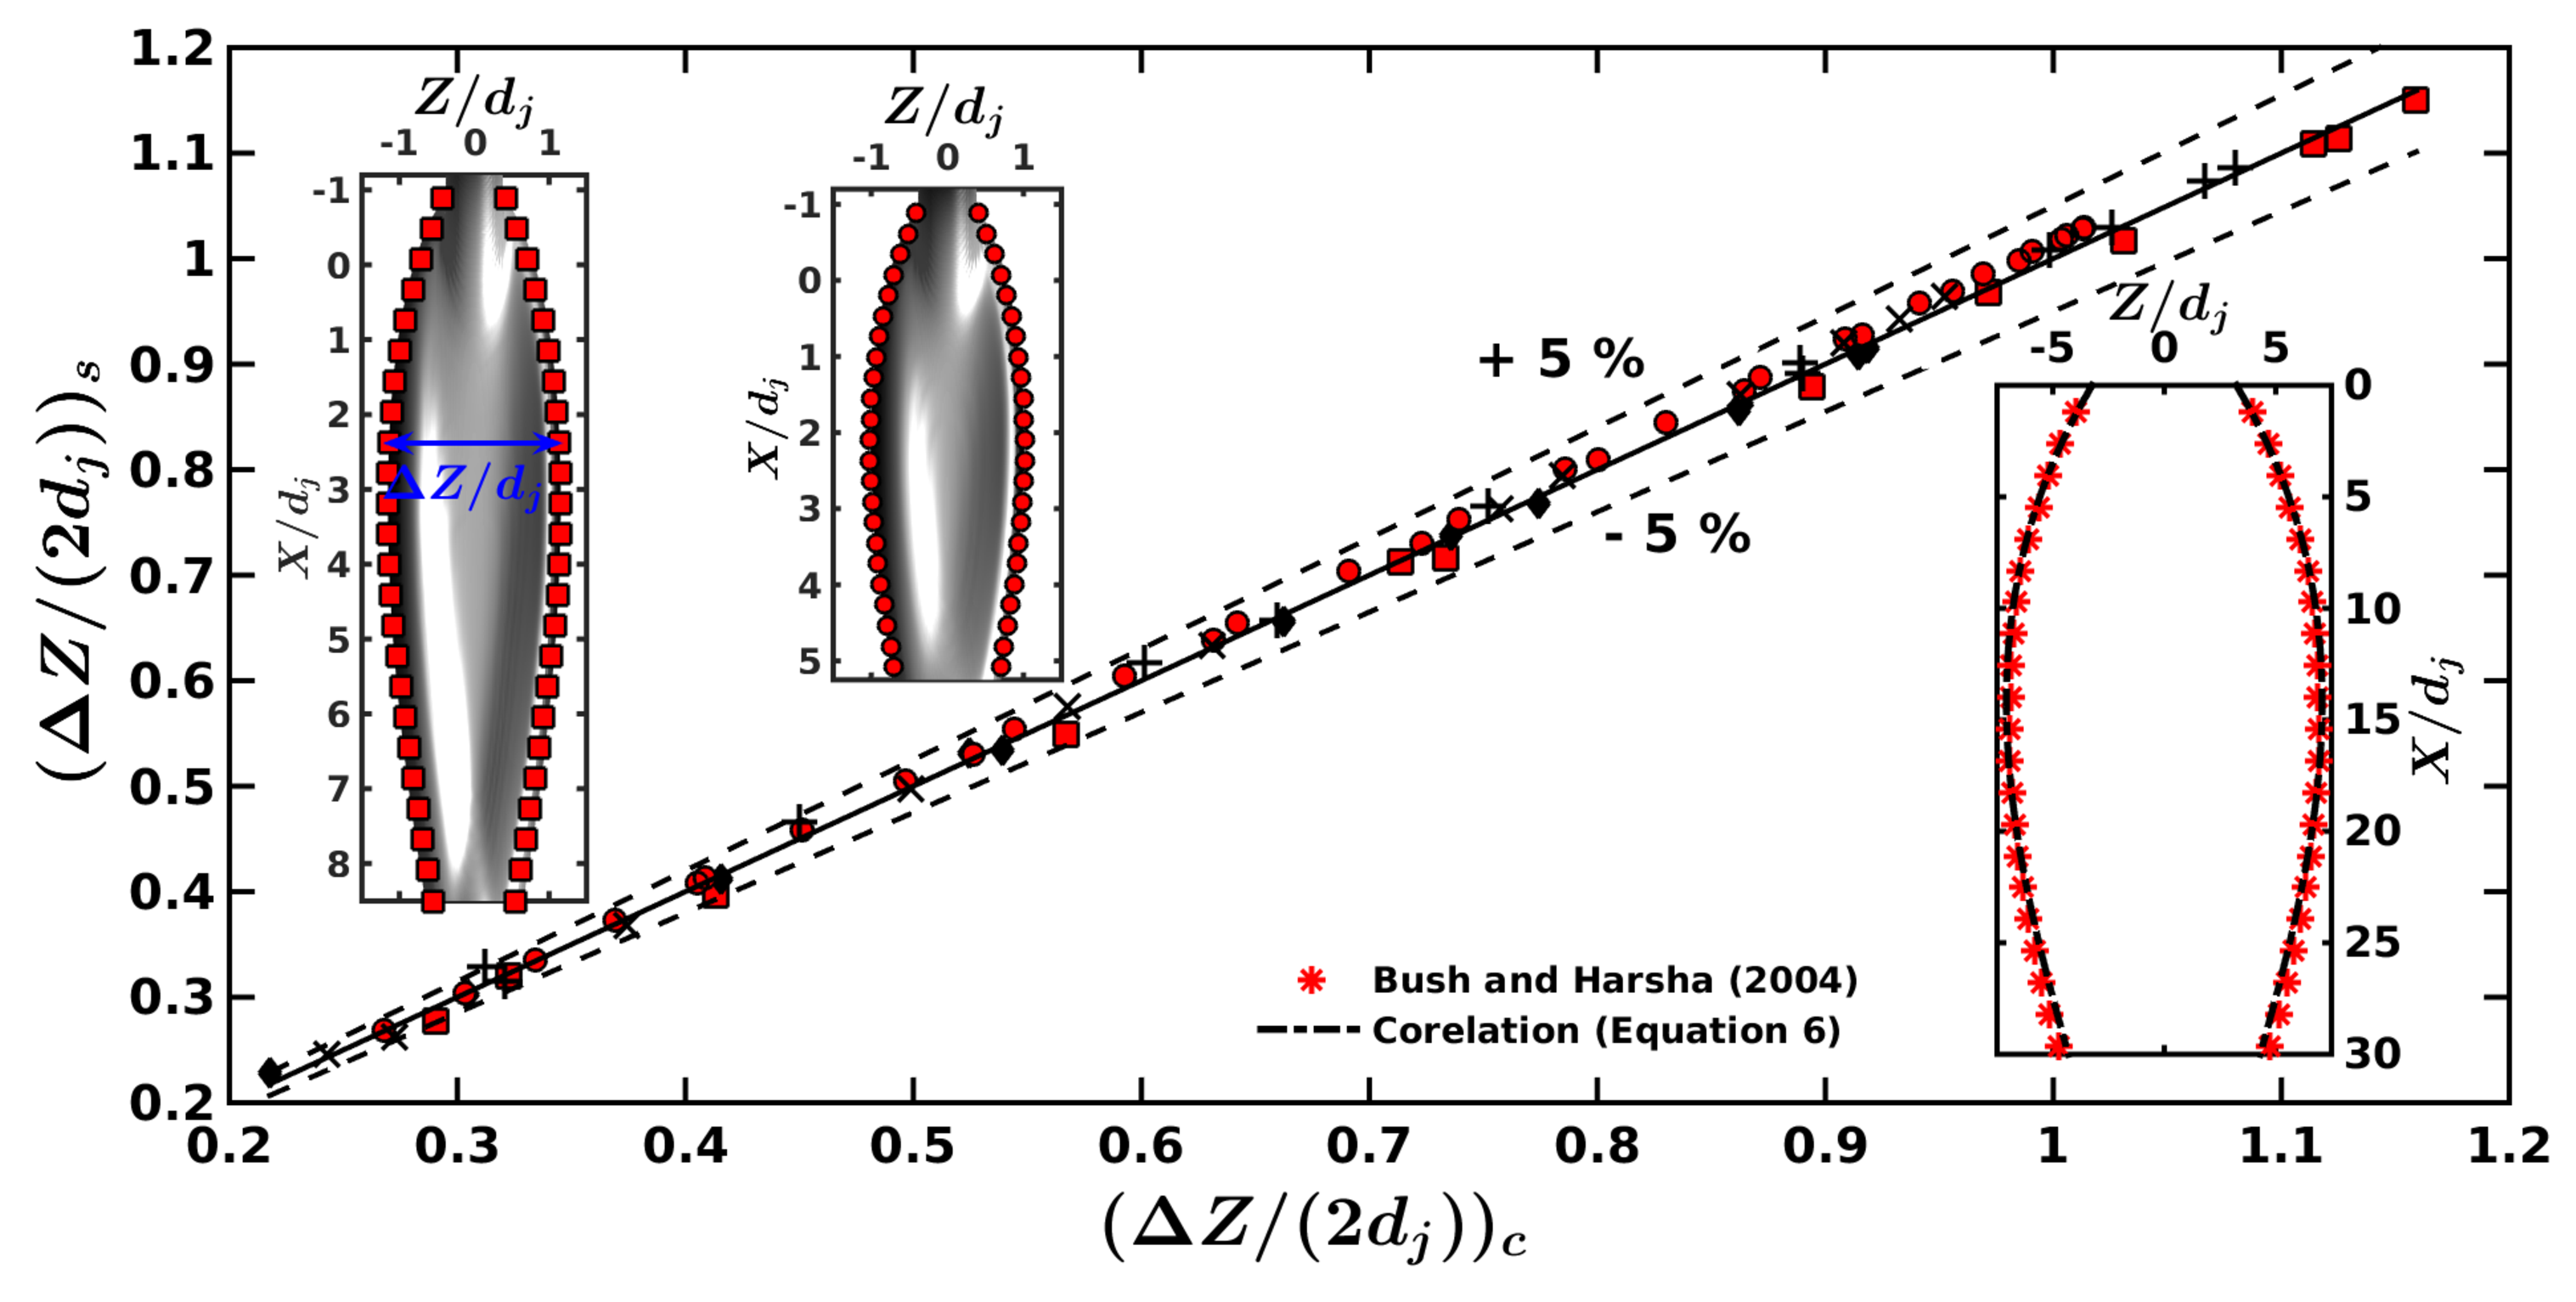
\includegraphics[width=\linewidth]{Figure9}
	\caption{Comparison between the values of expansion of the sheet outer periphery $\left(\Delta Z(x)\right)$ as predicted from equation~\ref{Equation::correlation} and from numerical simulations for different test cases with (symbol, $\alpha$, $Fr$, $Bo$, $Re/Fr$) = (\protect\MarkerSquareRed, 30$\degree$, 2.5, 5, 34); (+, 30$\degree$, 2.5, 4, 34); (\protect \MarkerDiamondBlack, 30$\degree$, 2.5, 2.3, 20); ($\times$, 25$\degree$, 2.5, 4.57, 34) and (\protect \MarkerCircleRed, 30$\degree$, 2.5, 3.75, 20). The first two inset figures (from the left) visualizes the corresponding three dimensional structure of the first link for the primary link and the third inset depicts the comparison between the equation~\ref{Equation::correlation} and the results of \cite{bush2004collision}.}
	\label{Figure::polyfit}
\end{figure*}
\begin{table}
	\centering
	\caption{Factors $\left(C_{m,n}\right)$ involved in equation~\ref{Equation::CorelationCoefficeints} determined by linear regression analysis to find the polynomial coefficients of equation~\ref{Equation::correlation}.}
	\label{Table::polyfit}
	\begin{tabular}{@{}cc|ccccccccc@{}}
		&   &     &   & & &n &      &    &   &        \\
		& $C_{m,n}$  & 0 &   &  & 1 &      & 2 & &   & 3      \\\hline
		& 0 & ~3.662&  & & ~2.720&  & ~0.353& & & ~0.512  \\
		& 1  & -0.082 &&  & ~0.490  & & ~1.146& & & ~0.592  \\
		m& 2 & -2.166 & & & -0.940& & ~0.408& & & ~0.761  \\
		& 3 & -1.504& & & -0.831& & ~0.074& & & -0.065 \\
		& 4 & -0.657& & & -0.290& & ~0.029&& & ~0.039  \\ 
	\end{tabular}
\end{table}
Efforts are also made to relate polynomial coefficients $\left(p_n\right)$ with non-dimensional numbers using linear regression analysis. Hence, $p_n$ can be expressed as
\begin{equation}\label{Equation::CorelationCoefficeints}
p_n = C_{0,n}\left(\sin\alpha\right)^{C_{1,n}}\left(Fr\right)^{C_{2,n}}\left(Bo\right)^{C_{3,n}}\left(Re\right)^{C_{4,n}}
\end{equation}
Values of $C_{m,n} \left(\forall\:\: m \in {0,4}\right)$ in equation~\ref{Equation::CorelationCoefficeints} are tabulated in the table~\ref{Table::polyfit} obeying $R^2$ norm of regression higher than 0.925. Predictability of the correlation with numerical chain contours are shown in the insets of figure~\ref{Figure::polyfit} for two different cases of non-dimensional numbers. It can be also observed from figure~\ref{Figure::polyfit} that the developed correlation gives a very good match ($\pm$5\%) with the numerical sheet profiles. So as to check the capability of the correlation, for prediction of experimental profiles of the chain structure, the comparison is made between observation of \cite{bush2004collision} and equation~\ref{Equation::correlation}. The reported excellent match in the inset of figure~\ref{Figure::polyfit} confirms the universality of the developed correlation. It is essential to understand the formation physics of widely influenced sheet structure generated due to the collision of jets. Next section dedicatedly discusses the issue.
\section{Analogy of chain formation}	
To bring out the physical insights of the liquid jet collision, idealizations are made for tracing back the sheet profile as a result of the collision between a train of fluid quanta (each of mass $m$), analogous to jet, in the plane of the sheet. It is assumed that the fluid quantum in a given jet interacts only with its mirror image in the other jet and that they are non-deformable. The collision is taken as friction-less. However, the follow-up trajectory of these fluid parcels after the collision is considered damped so as to mimic resistive forces like viscous and surface tension. A free body diagram and schematic of the fluid quanta collision assumption to replicate the sheet structure is depicted in figure~\ref{Figure::analytical}(a). Apart from inertial and gravitational forces, on the fluid particle, a damping force of magnitude $f_n$ (to impose the effect of viscous dissipation and surface forces) is also attached in the direction perpendicular to the individual packet's instantaneous velocity, post-collision. Absence of these resistive forces will make infinitely stretched sheet \citep{taylor1960formation}, with $f_n$ = 0 case. In-situ assessment of damping force based on local velocity may improve the prediction of resistive forces which has not been targeted in the present effort. Reference frame for the trajectory of the fluid quantum ($\zeta$) is considered to have the origin at the point of collision with $\zeta$ = 0 at $X$ = 0. Free body force analysis of the fluid particle, post-collision can be expressed as equations~\ref{Equation::tangential} and~\ref{Equation::normal}, with accelerations $a_n$ and $a_t$ in normal ($n$) and tangential ($t$) directions respectively.
\begin{subequations}%
	\label{Equation::forceBal}	
	\begin{eqnarray}
	\label{Equation::tangential}
	\text{Direction t:}\:\:\: a_t = v_{q}\frac{dv_{q}}{ds} &=& g\cos\phi\\
	\label{Equation::normal}
	\text{Direction n:}\:\:\: a_n = g\sin\phi + \frac{f_n}{m} &=& \frac{v_{q}^2}{r_c}
	\end{eqnarray}
\end{subequations}
\begin{figure*}
	\centering
	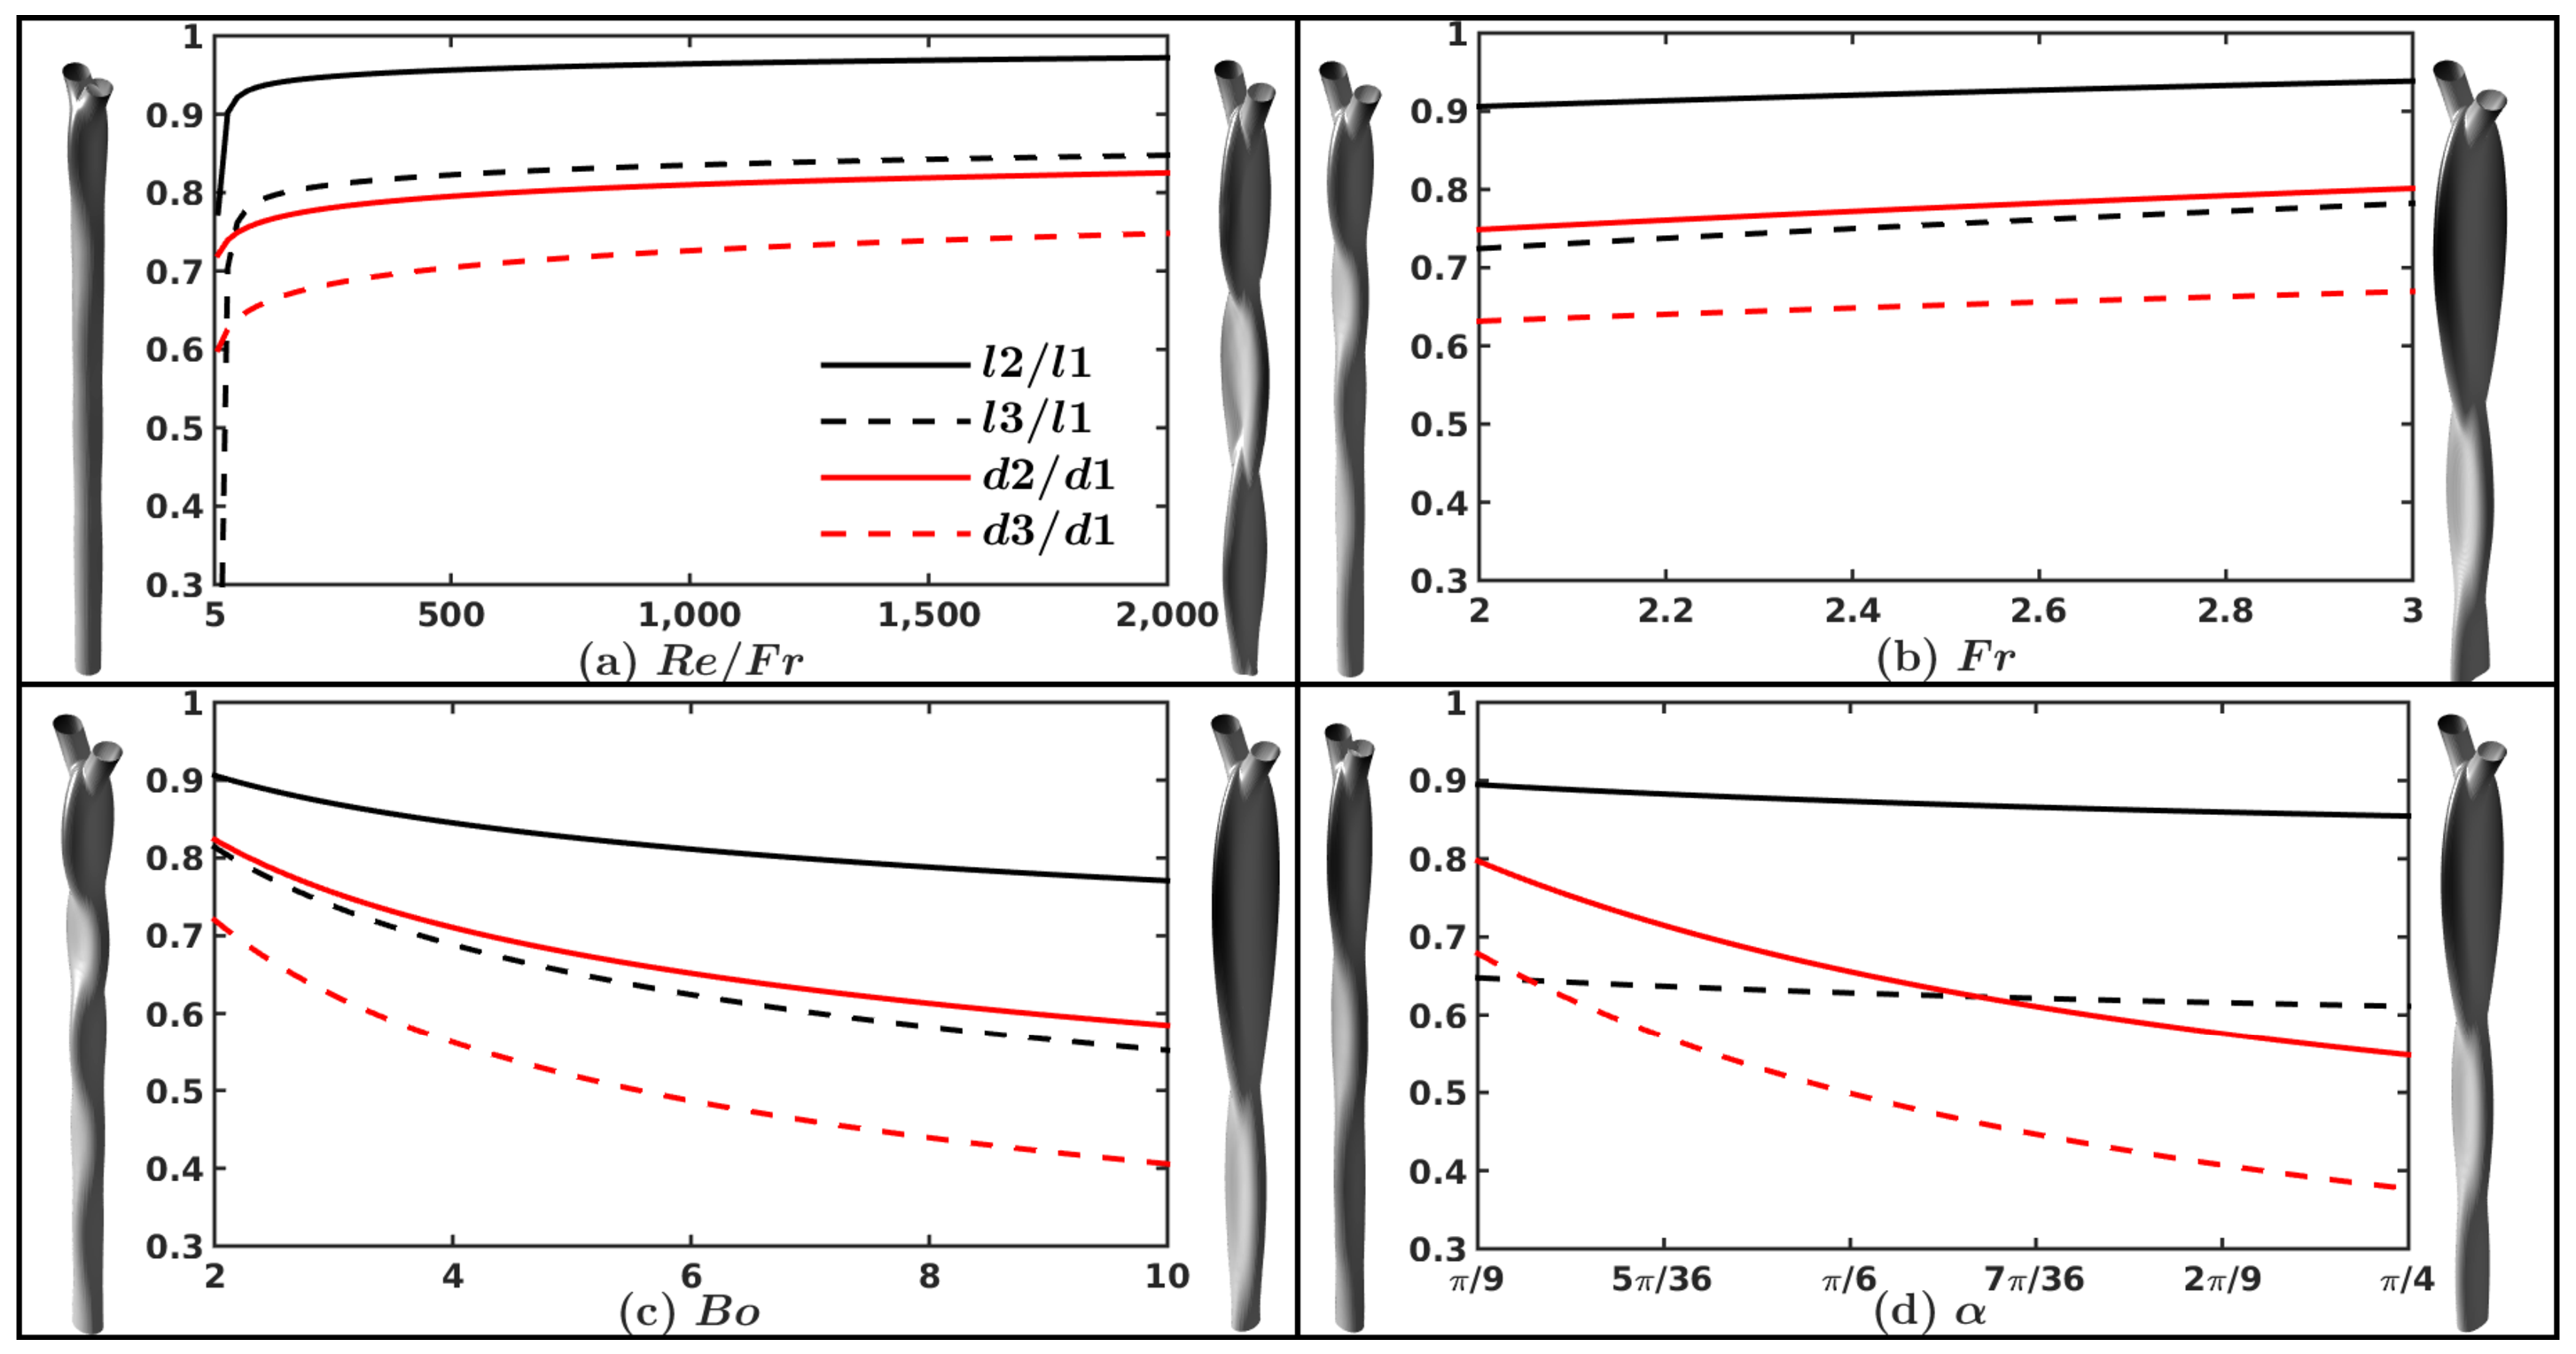
\includegraphics[width=\linewidth]{Figure10}
	\caption{Fluid quanta collision analogy: (a) schematic of the model and free-body diagram and comparison between the link shape obtained through numerical simulations and the fluid quantum trajectory ($\zeta$, \protect\MarkerSquareRed) for ($\alpha$, $Fr$, $Re/Fr$, $Bo$) = (a) (30$\degree$, 2.5, 34, 5), (b) (30$\degree$, 2.5, 23, 3.85), (d) (30$\degree$, 2, 34, 4.56) and (e) (45$\degree$, 2, 34, 3.4).}
	\label{Figure::analytical}
\end{figure*}%
Here, $r_c$ is the radius of curvature in $\zeta-X$ plane and $\phi = \tan^{-1}\left(\frac{d\zeta}{dX}\right)$. Integrating tangential momentum equation with increment $ds = dX/\cos\phi$ along with boundary condition at $X$ = 0, instantaneous fluid particle velocity ($v_{q}$) can be obtained as $\sqrt{u_j^2 + 2gX}$. Rearrangement of momentum equation in the normal direction after defining $\Lambda$ as $\frac{f_n}{mg}$ and inertial length scale, $\chi$ equivalent to $\frac{u_j^2}{2g}$, one obtains:
\begin{equation}\label{Equation::Final1}
r_c\left(\sin\phi + \Lambda\right) = 2\chi\left(\frac{X}{\chi} + 1\right)
\end{equation} 
After necessary integration, equation~\ref{Equation::Final1} simplifies to:
\begin{equation}
\sin\phi  = \sin\alpha + \left(\Lambda + \sin\alpha\right)\left(\frac{1}{\sqrt{\frac{X}{\chi} + 1}} - 1\right)	
\end{equation}
Recalling that $\tan\phi = \frac{d\zeta}{dX}$ and expressing $\Lambda/\sin\alpha = \eta$, profile of fluid quantum movement can be characterized as:
\begin{equation}
\label{Equation::AnaFinal}
\frac{d\zeta}{dX} = \tan\left\lbrace\sin^{-1}\left[ \sin\phi_0\left(1 + \eta\right)\left(\frac{1}{\sqrt{\frac{X}{\chi} + 1}} - 1\right) \right]\right\rbrace
\end{equation}
The functional form of the fluid particle trajectory, the equivalence of sheet profile, can be integrated numerically to obtain the coordinate points in the $\zeta-X$ plane after tuning only control factor, $\eta$ from some simulated profiles. In this process, $L^1$ relative error norm is kept below 10\%. Efforts have been also made to express control parameter, $\eta$ in terms of non-dimensional numbers for the range of values presented in this work. With 99\% $R^2$ regression norm, $\eta$ can be related with non-dimensional numbers as:
\begin{equation}\label{Equation::eta}
\eta = 3.28(\sin\alpha)^{-0.077}(Fr)^{0.502}(Bo)^{-0.248}\left(Re\right)^{-0.084}
\end{equation}
Proposed concept of collision of fluid quanta for mimicking the sheet profile is also tested with phase contours of numerical simulations. Some representative matches are shown in figures~\ref{Figure::analytical}(b) -~\ref{Figure::analytical}(e) in connection of primary link. Fundamental analysis of forces, a single controlling parameter in sheet profile (equation~\ref{Equation::AnaFinal}) and an excellent match with numerical data supplies in-depth knowledge about the formation of the liquid chain. Next, we focus on the mutual relationship between links formed at successive orthogonal planes. 
\section{Inter-relation between inter-connected links} 
\begin{figure}
	\centering
	\includegraphics[width=0.5\linewidth]{Figure11}
	\caption{Inter-relation between links of chain reproduction of secondary link of Case 1 ($\alpha$ = 30$\degree$, $Fr$ = 2.5, $Bo$ = 4, $Re/Fr$ = 34) as primary link of case 2 ($\alpha$ = 25$\degree$, $Fr$ = 2.2, $Bo$ = 4, $Re/Fr$ = 34) and tertiary link of Case 1 as secondary link of Case 2 and primary link of case 3 ($\alpha$ = 11.25$\degree$, $Fr$ = 1.98, $Bo$ = 4, $Re/Fr$ = 34) using (a) three dimensional chain structure and (b) two dimensional planar link locations.}
	\label{Figure::secondCollision}
\end{figure}
\begin{figure*}
	\centering
	\includegraphics[width=\linewidth]{Figure12}
	\caption{Generalization of fluid rim collision for the higher order links with the prediction of angles of impingement for (a) secondary and (b) tertiary collisions and (c) the account of rim strength ($Fr$) in different links.}
	\label{Figure::secondGraph}
\end{figure*}
\begin{figure*}
	\centering
	\includegraphics[width=\linewidth]{Figure13}
	\caption{Evaluation of the dimensional characteristics of the secondary and tertiary links relative to the primary link, for variations of (a) $\alpha$ at $Fr$ = 2.5, $Bo$ = 4.57 and $Re/Fr$ = 34 (b) $Fr$ at $\alpha$ = 30$\degree$, $Bo$ = 3.4 and $Re/Fr$ = 34 (c) $Bo$ at $\alpha$ = 30$\degree$, $Fr$ = 2.5 and $Re/Fr$ = 34 and (d) $Re/Fr$ at $\alpha$ = 30$\degree$, $Fr$ = 2 and $Bo$ = 3.4.}
	\label{Figure::secondLink}
	\vspace{-0.5mm}
\end{figure*}
The secondary and tertiary links observed in mutually perpendicular planes initiate with the collision of rims in preceding links. From our numerous simulations in the wide range of operating parameters, it can be observed that secondary, tertiary and subsequent links of a chain are equivalent to primary, secondary and subsequent links of another chain having different operating parameters. Hence, it is proposed that subsequent links are equivalent to resultant of collision between two free jets having reduced strength. To prove our  assumption, for example in figure~\ref{Figure::secondCollision}(a), a representative chain structure is identified for $\alpha$ = 30$\degree$, $Fr$ = 2.5, $Bo$ = 4, $Re/Fr$ = 34 (Case 1), in which secondary links showed resemblance with primary link of $\alpha$ = 25$\degree$, $Fr$ = 2.2, $Bo$ = 4, $Re/Fr$ = 34 (Case 2). Continuing this one can also establish analogy among tertiary link of Case 1, secondary link of Case 2 and primary link of $\alpha$ = 11.25$\degree$, $Fr$ = 1.98, $Bo$ = 4, $Re/Fr$ = 34 (Case 3). One to one correspondence of these links of different cases establishing present proposal is shown in the comparative graph of figure~\ref{Figure::secondCollision}(b). It can be commented that subsequent links are reduced in size, giving a feeling of resultant of impact between two weaker jets. The analogy between interconnected links in a chain and one level lower link of another chain is found to be valid with $\pm$ 10\% confidence for the entire region of search space of the operating parameters ($\alpha$, $Fr$, $Re/Fr$, $Bo$). A critical assessment of links in chain structure and rim profile has also established that angle of impingement between rims successively reduces $\alpha_{n}/\alpha_{n-1} < 1 \:\:\forall\:\: n = 1, 2, 3 \:\:\text{and higher integers}$. It has been also checked that analogy of collision between fluid parcels and formation of the link by the interaction between rims is also valid after taking the reduction of angle of impingement into consideration. This trend is shown in the figures~\ref{Figure::secondGraph}(a) -~\ref{Figure::secondGraph}(b) for secondary and tertiary links for few chain cases randomly scattered in search space. With only $\pm$ 10\% error, theory of collision between the fluid quanta (equations~\ref{Equation::AnaFinal} -~\ref{Equation::eta}) has also found to be applicable for $n^{th}$ order link of chain. Polynomial proposed in equation~\ref{Equation::correlation} also predicts formation of $n^{th}$ order link satisfactorily with modified strength and impingement angle. Clustering of points near (1,1) for secondary link (figure~\ref{Figure::secondGraph}(a)) and (0,0) for tertiary link (figure~\ref{Figure::secondGraph}(b)) establishes continuous reduction of impingement angle $\alpha_{n}$ with increase in link number $n$. Besides the reduction in angle of impingements, the interaction between rims of a link can be also considered as the collision between jets of lesser Froude number ($Fr_m$) than $Fr_j$. The monotonous decrement of $Fr_m$ is observed as one traverses in subsequent higher level links along a chain. Figure~\ref{Figure::secondGraph}(c) establishes this idea where the ratio between rim Froude number of secondary link ($Fr_2$) to jet Froude number ($Fr_j$) has been fitted as 0.88 and that of same for the tertiary link ($Fr_3/Fr_j$) as 0.8. These decrements are a result of the viscous dissipations which are prominent at the time of the collision and has been illustrated in figure~\ref{Figure::secondLink} (with the extreme cases of variations shown as insets figures across each graph) for the entire domain of non-dimensional numbers considered in the present work. The dimensional characteristics of the secondary and tertiary links are studied as relative to the primary link. The range of values of $l_i/l_1$ and $d_i/d_1$ is always less than 1. Further, it must be noted that the final resultant liquid jet formed after the diminishing of chain structure also shows some undulations on its surface. Therefore, we have considered the presence of higher order links only if the difference in relative dimensional characteristics is more than 30$\%$. For fluids with higher viscosities, the formation of this resultant jet is most prominent as shown in figure~\ref{Figure::secondLink}(a). As the viscosity is decreased ($Re$ is increased), there is a sudden increase in the dimensional characteristics because of the reduced viscous dissipations at the time of collision of subsequent rims of the sheet. However, similar to the effects of $Re$ on single link dimensions, this influence saturates after the initial increase as for the less viscous fluids (high $Re$), the formation of chain structure is surface tension and inertia driven. Further, with an increase in the inertia of the liquid jets, the individual links grow in size but because of the viscous dissipations, this effect is not transmitted equally downstream of the flow. The second link also increases in dimensions but the length and width of the second link are always smaller than the primary link (figure~\ref{Figure::secondLink}(b)). Moreover, an increase in the $Bo$ (decrement in the surface tension coefficient of the interface), the length and width of the first link increase substantially \citep{yang2014liquid,bremond2006atomization}. As a result, the primary sheet thickness and the rim diameter decrease leading to the reduction of the inertia of the rims responsible for the secondary and subsequent collisions. Therefore, the dimensional characteristics of the higher order links as compared to the first one decreases with an increase in $Bo$ (figure~\ref{Figure::secondLink}(c)). A similar decrement in also observed if the angle of impingement is increased (figure~\ref{Figure::secondLink}(d)) as the primary link grows faster in size than the others. Though the idea of the interrelation between the links is established only for first three, it can be extrapolated for higher order elements in the chain until it transforms into a jet.

\section{Conclusion}
The stable chain structures are formed by the collision of laminar liquid jets when the inertia forces are, in order of magnitude, similar to the surface tension forces. A series of fully resolved numerical simulations showed that individual links, formed by collision of cylindrical jets (primary) or rims (secondary onward), occupy mutually orthogonal planes with a successive reduction in size owing to viscous effects. The fluid parcels inside these links are dispatched radially outwards from the stagnation point and follow trajectories self-similar to the phase boundary. The variation of the velocity field across the radial coordinate is found to be negligible whereas the azimuthal variation of the sheet velocity is scaled using its average, given by an empiric relation. Further, at the collision planes, the velocity field is found to be retracting in the direction of the colliding jets and rims whereas it is expanding in the plane of the formed sheets. The inertial and gravitational forces provide a measure of the expansion of these sheets counteracted by the surface tension at the interface and viscous dissipations at the subsequent collisions. An increase in the impingement angle ($\alpha$) leads to wider links of the chain with a negligible change in the length of individual links. Intuitively, the size of the stable chain structure increases with an increase in the momenta of the jets ($Fr$) or with a decrease in the strength of the surface tension force (increasing $Bo$). Increase in the $Re$ presents a sharp increase in the dimensions of the chain, which saturates at the higher values of $Re$. Moreover, the individual symmetric sheet profile can be modeled using a third order polynomial, with an accuracy of $\pm$ 5\%, with coefficients dependent on various non-dimensional numbers featuring the interplay of different forces. Effects of these forces have been understood by mimicking them onto the post-collision trajectory of fluid quanta. Higher order links are found to be similar to lower or primary level element formed due to impact between jets of reduced $Fr$ and $\alpha$. 

\section{Supplementary material}
See supplementary material for the complete movie of the time sequenced still images provided in figure~\ref{Figure::temporal} showing the formation of a liquid chain.

\bibliography{chainPaper}% Produces the bibliography via BibTeX.

\end{document}
%
% ****** End of file aipsamp.tex ******
